% 文件名:MainBody.tex
% 文件描述:以 scuthesis 四川大学学位论文文档类为基础的 LaTeX 模版
% 作者:LegendaryLeo
% 修改日期:2019年5月3日
% 选用scuthesis文档类,参数master为硕士论文,可选doctor和bachelor,分别对应博士和学士
\documentclass[bachelor,UTF8,hyperref]{./Template/scuthesis}
\usepackage{fancyvrb}
\usepackage{xcolor}
\usepackage{dirtree}
\usepackage{textcomp}
\renewcommand*{\DTstylecomment}{\color{blue}\kaishu}
\usepackage{supertabular}
\usepackage{longtable}
\usepackage{graphicx} % 插入图片
\usepackage{float} %设置图片浮动位置的宏包
\usepackage{subfigure} %插入多图时用子图显示的宏包
\usepackage{listings}
\usepackage{makecell}
%\newcommand{\supercite}[1]{\textsuperscript{\cite{#1}}}
\begin{document}
% 设置文档信息
\title{图书异地租借系统}
\ENGtitle{Books Off-site Rental System}
\CoverTitle{图书异地租借系统} %封面标题
\author{邓雪}
\ENGauthor{DengXue}
\accomplishdate{2019年5月}
\school{计算机学院}
\supervisor{蒲蔚\quad教授}
\ENGsupervisor{Lecturer. Pu Wei}
\major{物联网工程}
\ENGmajor{Internet of Things Engineering}
\direction{物联网}
\ENGdirection{Direction Name}
\defensedate{2019.05}
\keywords{图书馆;异地租借;物流;web系统}
\ENGkeywords{Libray; Off-site rental; Express; Web System}
% 设置论文正文前的页码、页眉等
% 自动制作标题
\maketitle
\frontmatter\pagenumbering{Roman}\pagestyle{fancy}\makechaptertitlecenter
% 包含摘要
%!TEX root = ../MainBody.tex

% 中英文摘要
\begin{CHSabstract}
	本系统是传统图书管理系统的功能扩展和增强。通过对使用本校图书馆系统的师生调研、预约模块的功能分析,了解到当下预约借书功能的一些不足——不支持异地租借。为了满足读者这一可优化需求,研发本系统来完善书籍租借服务。功能上,提供线上预约,通过第三方物流体系,将书籍通过物流送达至目的地,跨越空间障碍,便于读者远程预约,提高实体图书资源利用率,同时合理开发与配置馆藏信息资源,进一步实现图书服务多元化。

	本系统基于B/S架构,使用React+Typescript+MobX+Webpack前端框架,基于MVVM设计模式,结合Node+Koa后端服务和文档型数据库MongoDB。提供读者端和管理员端。读者服务实现登录注册、查看图书列表和详情信息、预约借书、还书操作、物流信息管理等功能,管理员模块实现管理员登录、查看书籍预约信息,借还登记等功能。在上述基础功能的前提上,提供物流通知、书籍推荐,消息推送至流媒体、社交网络等功能,实现系统的横向扩展。通过权限控制,安全防护和防抖节流来提高系统稳定性。同时,优化页面细节和数据库设计,增强系统易用性,优化用户体验。
\end{CHSabstract}
\begin{ENGabstract}
This system is a extension and enhancement of the traditional library management system. Through the analysis of the functions of the library system and the readers' research, we learned about the problems in the current borrowing process, and in order to meet the needs of readers, we developed this system to improve the book lending service. Functionally, online reservations are provided. Through the third-party logistics system, books are delivered to destinations through logistics, which overcomes space barriers, facilitates readers to borrow, improves the utilization of library resources, and rationally develops and configures information resources to realize the diversity of book services. Chemical.

The system is based on Browser/Server architecture, MVVM design principle, using React+Typescript+MobX+Webpack front-end framework, Node+Koa backend service and document database MongoDB. Provide reader service and administrator services. The reader service implements functions such as login registration, viewing book list and detailed information, borrowing and returning operations, personal information management, etc. The administrator module implements functions such as administrator login, viewing book reservation information, and borrowing registration. On the premise of the above basic functions, it provides logistics notification, book recommendation, message push to streaming media, social network and other functions to achieve horizontal expansion of the system. Improve system stability through access control, security and anti-shake throttling. At the same time, optimize page details and database design to enhance system usability and optimize user experience.
\end{ENGabstract}

% 包含缩略词表
% %!TEX root = ../Manual.tex
\chapter{常用缩略词表}
\emph{例:}\par
\begin{table}[ht]
	\centering
	\begin{tabular*}{\textwidth}{|p{0.3\textwidth}|p{0.7\textwidth}|}
		\hline
		TUG & \TeX~ Users Group       \\
		bib & Bibliography            \\
		bst & Bibliography Style      \\
		def & Define                  \\
		toc & Table of Contents       \\
		eps & Encapsulated PostScript \\
		cls & Class                   \\
		SCU & Sichuan University
	\end{tabular*}
\end{table}

% 包含符号表
% \include{Chapters/0_2_Symbols}
% 自动制作目录
\maketoc
% 设置论文正文部分的页码、页眉等
\mainmatter\pagenumbering{arabic}\pagestyle{fancy}\makechaptertitleleft
% 包含第一章、第二章等等
%!TEX root = ../MainBody.tex

% 第一章
\chapter{绪论}
% 以上为一级标题——绪论,此处为一级标题正文。参考文献引自\cite{tlc}。
% \section{二级标题}
% 此处为二级标题正文。
\section{背景}
现有的图书管理/租借系统大多并不支持线上借书服务。这意味着读者在网页端或微信端预约借书后,需要到馆内才能取得书籍。这一方式存在一些问题,如寒暑假期间、读者出差在外、由于学业或工作繁忙等原因,无法亲自到馆借书,希望能够通过图书快递的方式,直接将书籍配送到读者所在地址。
这一门槛可能把大多数有阅读需求的读者拒之门外,本系统研发的初衷便在于解决这一问题,打通物流,跨越读者与图书的空间障碍,改善借阅方式,打造"读者-web端-物流-图书"模式,满足读者的多元化需求。另外,由于阅读具有非强制性,大部分租借系统也存在利用率低下的问题,部分可能从中受益的读者可能并没有接触使用,可以通过扩展系统的社交属性,将消息推送至主流社交媒体等方式,一定程度上缓解这一问题。
\section{选题意义}
\begin{enumerate}
    \item 有利于提高纸质图书利用率。在校内图书馆系统现有功能基础上,增加图书异地租借服务,支持图书邮寄,主要解决假期期间学生借书困难的问题,同时也方便有校外借书需求的学生和教职工,进一步提高图书馆海量资源的利用率。
    \item 有利于提高师生综合素养。图书是知识、信息传播的重要载体,通过阅读能不断完善个人知识体系,建立正确的人生观、世界观、价值观。本系统支持pc端和移动端web访问,采用流式布局,界面简洁友好。在基础功能实现的基础上优化用户体验,是获取图书资源的优质渠道。有一定推广阅读的作用,配合图书馆系统现有的推荐服务,发挥图书其潜在价值,对提升师生阅读综合素养有所裨益。
    \item 有利于合理开发与配置信息资源,实现图书服务多元化。图书租借系统下要求对图书信息资源的开发与配置具备新观念和新方式。有利于结合当下图书借阅的实际情况,切实提升图书馆的服务水平和服务质量;其次,有助于多层次、联合式地开发和利用信息资源。从重视理论性资源开发逐步过渡到重视实践性和生活性的信息资源开发,从而可以满足用户的不同信息需求。
    \item 有利于推动图书相关研究进展。本系统可为相关大数据挖掘及分析工作提供可靠真实的图书借阅数据,推动此类研究的推进和发展。    
\end{enumerate}
\section{国内外研究现状}
近年来,随着计算机技术和网络技术的迅速崛起,互联网、“互联网+”模式的广泛应用日渐深刻的改变着人们的生产生活方式。互联网逐步进入传统的流通领域,电子商务开始流行,而物流则是电子商务中的重要一环。如今发达的互联网物流系统大大便捷了人们的日常生活,利用它的强大特性,作为图书租借系统的支持,能有效提高资源的流通和利用。

​国内外数字图书馆的实践活动大致可以分为以下三种类型: 服务研究型、资源服务型,联合建设型。虽然,从严格意义上讲,资源服务型不能算是数字图书馆,但它的网上信息服务目前已自大多数图书馆开展,是现阶段我国图书界提供网上数字服务的主要形式。

​目前,国内浙江省杭州图书馆和广东省深圳罗湖区图书馆已开通快递借书服务,读者可同时采用线上或线下方式借还书,另外还提供了读者优先选书功能,把图书采购和选择权在一定范围内交给读者,研发智慧图书系统,加强多平台信息共享,增加与读者之间的沟通交流,同时对读者的借阅数据进行分析,更好地明确读者的需求,主动推送更切合需求的书目。市民可通过图书馆借阅卡、实名认证或评估芝麻信用等方式进行认证,认证成功即可预约借书。


%!TEX root = ../MainBody.tex

% 第二章
\chapter{需求分析}% 使用\cite{}命令引用数据库中文献
\section{系统陈述}
本系统主要分为两个模块:用户模块和管理员模块。用户登录/注册成功,可进行查阅、借书、还书、查看个人的已预约书籍列表和代还列表,以及物流地址等其他个人信息。管理员登录成功后,可查看预约列表,包含所有用户的远程预约信息,并根据预约信息查找馆内对应的纸质书籍,通过物流送达至各个用户所填写的物流地址,快递员将书籍送到用户手中。部分异常情况,例如书籍遗失,如果是用户本人遗失书籍,按照现行纸质书遗失规定办法处理;如
果是物流配送方遗失书籍,由配送方赔偿损失。
\section{用户使用场景}
\subsection{场景一:用户借书}
场景名:用户在登录web端,选择书籍,借书。

参与者实例:Tony,用户;Steve,图书管理员。

场景:

Tony登录“图书异地租借系统”web端,浏览书籍列表,选择一本《百年孤独》,点击进入详情页,查看书籍简介和馆藏信息,当前书籍状态为可借阅,点击下方`预约借书`按钮,等待管理员确认。

Steve登录“图书异地租借系统”web管理端,点击待借列表,看到Tony的借书请求,在图书馆中找到书籍,同时交付给物流公司,将物流号填写到管理端上。

Tony在web端上可以看见管理员填写的物流单号,据此查询物流状态。快递员将书籍派送至Tony手中,Tony终于可以阅读了。
\subsection{场景二:用户还书}
场景名:用户还书,在web端点击还书按钮,并填写物流单号。

参与者实例:Tony,用户;Steve,图书管理员。

场景:

Tony看完《百年孤独》,准备还书,将书籍交付物流公司,并点击web端,进入"我的-待还书籍",页面显示所有待还书列表,Tony点击《百年孤独》那一行,在弹出页面中填写物流单号,点击确定。

Steve收到快递员寄来的图书时,确认书籍完好无损,使用馆的还书机器进行还书扫描,扫描成功后该书籍的状态自动更新为"已归还"。

Tony的待还列表更新,《百年孤独》这一行没有已经不在该列表中。
\section{用例建模}
\begin{figure}[H] %H为当前位置,!hpb为忽略美学标准,hpbp为浮动图形
    \centering %图片居中
    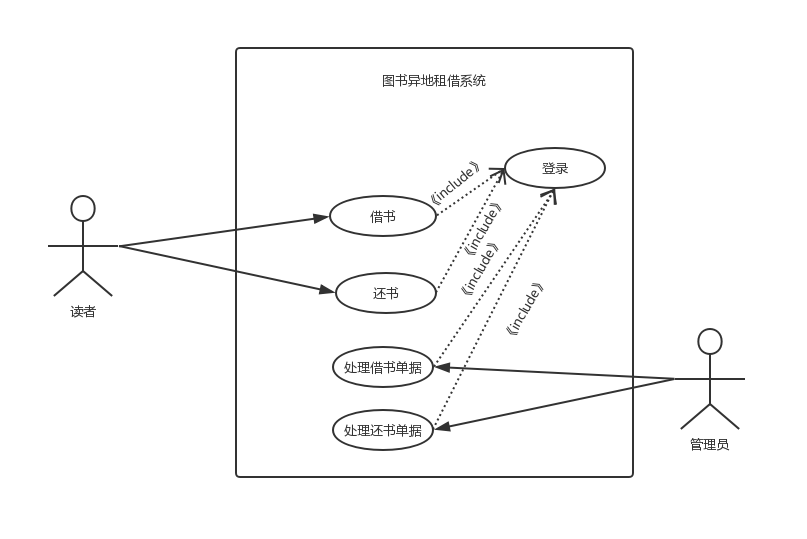
\includegraphics[width=0.7\textwidth]{./Chapters/images/example.png} %插入图片,[]中设置图片大小,{}中是图片文件名
    \caption{用例图} %最终文档中希望显示的图片标题
    \label{用例图} %用于文内引用的标签
\end{figure}
\begin{figure}[H] %H为当前位置,!hpb为忽略美学标准,hpbp为浮动图形
    \centering %图片居中
    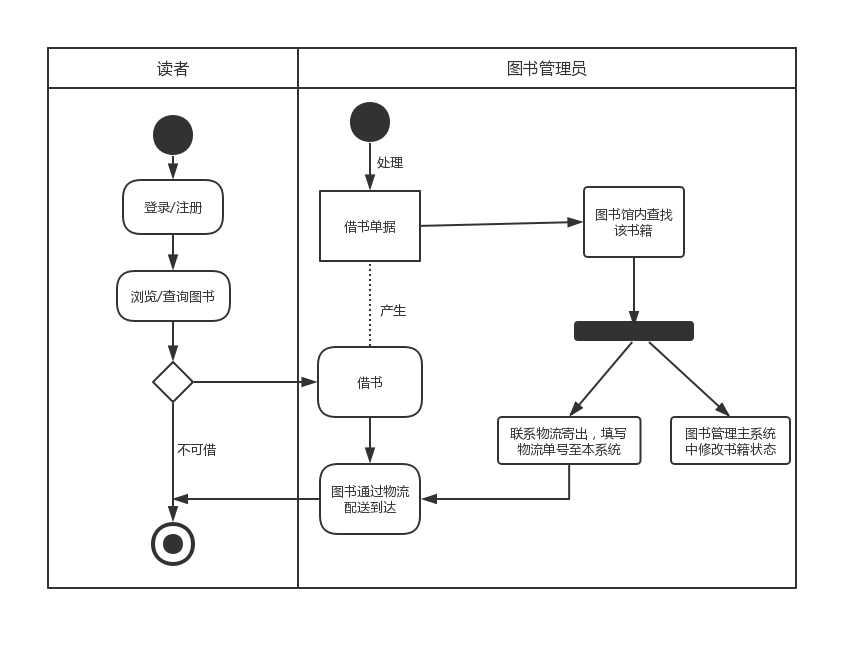
\includegraphics[width=0.7\textwidth]{./Chapters/images/activity.png} %插入图片,[]中设置图片大小,{}中是图片文件名
    \caption{活动图} %最终文档中希望显示的图片标题
    \label{活动图} %用于文内引用的标签
\end{figure}
\section{需求规约}
系统需求分为功能性需求和非功能性需求。功能需求可分为用户和管理员两大部分。对于用户来说,核心功能是在线预约书籍,书籍能够能通过物流方式送达。而管理员则主要是处理用户的预约请求,将书籍交付物流。
\subsection{功能性需求}
\subsubsection{用户相关的功能需求}
\begin{itemize}
    \item 登录/注册,登录的账号密码与借书卡的账号密码一致,读者注册于图书管理主 系统一致,需要到馆内注册借书卡,注册成功后,通过借书卡的账号/密码登录本系统。
    \item 图书列表展示,以图文卡片列表的方式展示图书馆馆藏书籍,卡片中包含书籍 的作者、出版社、简介等基本信息和借书条码号、可借数量及馆藏总数量等,可 借数量大于 0 时,读者可以点击预约按钮进行预约借阅。
    \item 借还书操作,在系统中的书籍列表和已预约列表中,可进行预约借书/取消预约 操作。在待还列表中可点击还书按钮,申请还书。
    \item 个人信息,包含物流地址信息、已预约书籍列表、待还列表等个人信息。
\end{itemize}
\begin{table}[hp]
    \centering
    \caption{用户登录}
	\begin{tabular*}{\textwidth}{p{0.25\textwidth}|p{0.7\textwidth}}
    \hline
    用例名称    & 用户登录                                                                                                                             \\ \hline
    用例描述    & 用户通过账号密码登录本系统的整个流程                                                                                                               \\ \hline
    执行者     & 用户                                                                                                                               \\ \hline
    前置条件    & 该用户拥有图书馆的借书卡,并知道借书卡的账号和密码                                                                                                        \\ \hline
    后置条件    & 生成有效期为7天的唯一登录token                                                                                                                             \\ \hline
    主事件流描述  & \begin{enumerate} 
            \item 用户在未登录(未登录规则参见业务规则a)的情况下,访问本系统的任意界面,系统自动跳转至登录界面;
            \item 用户输入持有借书卡的账号和密码,系统校验输入的账号和密码,应用业务规则b,若校验失败,执行异常过程2.1.1;若校验成功,系统自动跳转至主界面。
        \end{enumerate} \\ \hline
    分支事件流描述 & ~                                                                                                                                \\ \hline
    异常事件流描述 & 2.1.1 若不存在该账号,则系统提示该账号不存在;若账号和密码不匹配,则系统提示账号密码不匹配,返回2                                                                             \\ \hline
    业务规则    & a. 未登录状态可由2种情况判定:1. 用户第一次登录;2.  用户之前登录过,但登录token已失效 b. 先查询系统中是否存在该账号,不存在则校验失败,存在则校验账号和加密后的密钥是否与数据库中存储的数据匹配,不匹配则校验失败,匹配则校验成功.    \\ \hline
    涉及的业务实体 & 借书卡账号、密码                                                           \\ \hline
\end{tabular*}
\end{table}
\begin{figure}[H]
    \centering  %图片全局居中
    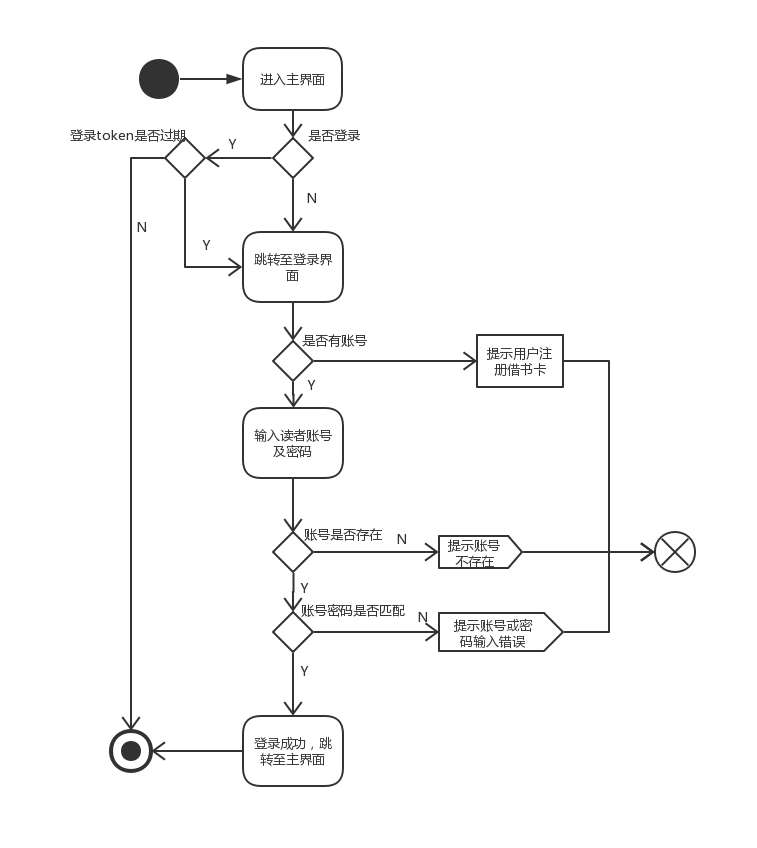
\includegraphics[width=0.45\textwidth]{./Chapters/images/activity_login.png}
    \caption{登录活动图}
    \label{登录活动图}
\end{figure}
%图书列表展示:
\begin{table}[hp]
    \centering
    \caption{浏览图书列表}
	\begin{tabular*}{\textwidth}{p{0.25\textwidth}|p{0.7\textwidth}}
    \hline
    用例名称    & 浏览图书列表    \\ \hline
    用例描述    & 用户进入主界面,浏览图书列表,查看图书信息    \\ \hline
    执行者     & 用户         \\ \hline
    前置条件    & 用户已成功登录本系统   \\ \hline
    后置条件    & ~     \\ \hline
    主事件流描述  & \begin{enumerate} 
            \item 用户进入主界面,系统显示书籍列表,每个列表项展示书籍封面、书名、可借数量、馆藏数量、预约按钮、详情按钮
            \item 用户点击借书,若书籍可借数量为0,应用业务规则a,否则执行分支过程2.1.1,若用户点击详情,执行分支过程2.2.1
        \end{enumerate} \\ \hline
    分支事件流描述 & \begin{itemize} 
        \item[2.1.1] 弹出二次确认框,点击确认则请求预约借书,取消则用例终止
        \item[2.2.1] 详情按钮上方弹出气泡,气泡中显示书籍简介信息
    \end{itemize}     \\ \hline
    异常事件流描述 & ~  \\ \hline   
    业务规则    &  a. 若预约按钮不可点击  \\ \hline
    涉及的业务实体 & 图书      \\ \hline
\end{tabular*}
\end{table}
% 借书操作
\begin{table}[hp]
    \centering
    \caption{借书操作}
	\begin{tabular*}{\textwidth}{p{0.25\textwidth}|p{0.7\textwidth}}
    \hline
    用例名称    & 借书操作    \\ \hline
    用例描述    & 用户进入主界面,浏览图书列表,进行借书操作    \\ \hline
    执行者     & 用户         \\ \hline
    前置条件    & 1. 用户已成功登录本系统;2. 所选择的图书可借数量大于0  
     \\ \hline
    后置条件    & 1. 系统生成预约记;2. 管理员可查看该预约记录;3. 提交预约申请后可撤销  
    \\ \hline
    主事件流描述  & \begin{enumerate} 
            \item 用户浏览图书列表,点击某本书左下角的借书按钮,应用业务规则a,若该本书的可借数量为0,执行1.1.1,若可借数量大于0,执行2,点击预约列表,执行4
            \item 用户点击借书按钮后,系统弹出二次确认框,点击取消,用例结束;点击确认,系统发起借书请求,执行3
            \item 若系统请求成功,借书按钮的文案变为“已预约”,点击按钮,执行3.1.1
            \item 用户点击“预约列表”之后,系统展示所有已预约书籍列表,点击取消按钮,执行3.1.1
        \end{enumerate} \\ \hline
    分支事件流描述 & \begin{itemize}
        \item[1.1.1]  按钮不可点击,用例结束
        \item[3.1.1] 弹出"是否取消预约"的二次确认框,确认则系统发起取消预约请求,用例结束      
    \end{itemize} \\ \hline
    业务规则    &  a. 若该本书的可借数量大于0,则借书按钮可点击;若该本书的可借数量为0,则按钮为不可点击状态  \\ \hline
    涉及的业务实体 & ~     \\ \hline
\end{tabular*}
\end{table}
%还书操作
\begin{table}[hp]
    \centering
    \caption{还书操作}
    \begin{tabular*}{\textwidth}{p{0.25\textwidth}|p{0.7\textwidth}}
        \hline
    用例描述    & 用户在系统上申请还书,并交付物流或到馆还书的流程。    \\ \hline
    执行者     & 用户      \\ \hline
    前置条件    & 1.用户将书籍交付物流公司,并获取到物流单号    2.用户成功登录系统,待还列表中有该待还书籍   \\ \hline
    后置条件    & 1. 用户本人未造成书籍为损坏或遗失     2.物流配送过程中,书籍未损坏或遗失  3.管理员更新书籍为已还状态    \\ \hline
    主事件流描述  & \begin{enumerate} 
            \item 用户进入系统主界面,点击待还列表,找到待还图书所在的具体行,若未申请过还书,执行2;若已申请过还书,执行3
            \item 点击"我要还书"按钮,页面显示弹出框,在弹出框内填写物流单号,点击确认,执行分支过程2.1.1
            \item 列表项显示上次成功提交的物流单号,点击"修改物流"按钮,页面显示弹出框,在弹出框中修改物流信息,点击确认,执行分支过程2.1.1
            \item 物流公司配送书籍至图书馆,若书籍在配送过程中损坏或遗失,执行异常过程4.1.1
        \end{enumerate} \\ \hline
    分支事件流描述 & 2.1.1 系统提交表单,若提交成功,生成历史单号;若提交失败,系统提示提交失败,页面停留在表单编辑页    \\ \hline
    异常事件流描述 & 4.1.1 书籍损坏,图书管理员收到图书后,应用业务规则a,按照图书馆现行书籍损坏赔偿制度向物流公司或用户索赔;书籍遗失,管理员按照现行图书遗失赔偿制度向物流公司索赔 \\ \hline                                                                            \\ \hline
    业务规则    &  a. 书籍损坏,读者上传照片等凭证,须管理员确认读者本人未损坏书籍,否则由读者赔偿。 \\ \hline
    涉及的业务实体 & 图书、物流单号    \\ \hline
\end{tabular*}
\end{table}
\begin{figure}[H]
    \centering  %图片全局居中
    \subfigure[借书活动图]{
    \label{借书活动图}
    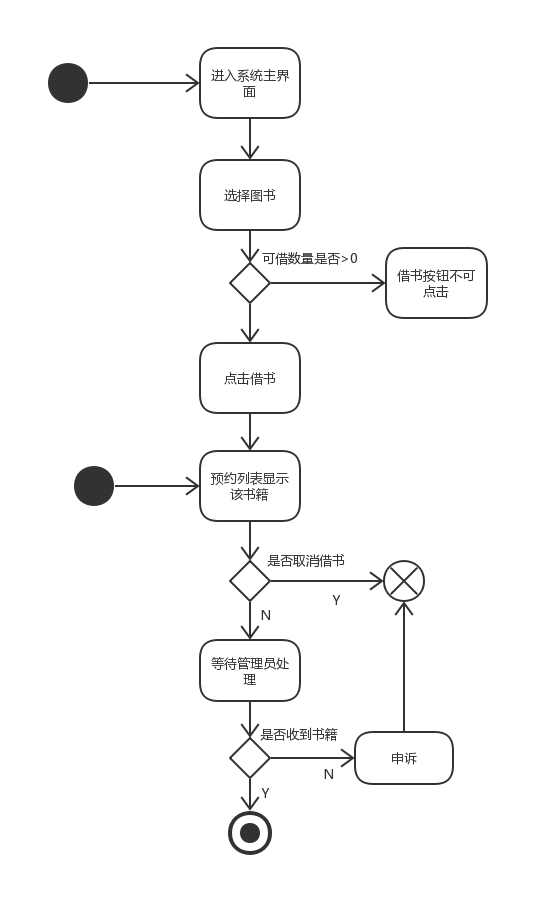
\includegraphics[width=0.45\textwidth]{./Chapters/images/activity_borrow.png}}
    \subfigure[还书活动图]{
    \label{还书活动图}
    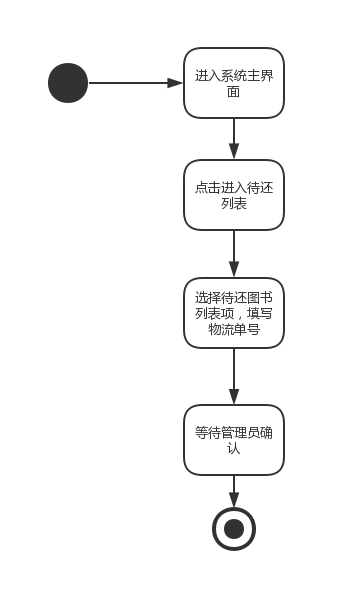
\includegraphics[width=0.45\textwidth]{./Chapters/images/activity_back.png}}
    \caption{借还书活动图}
    \label{借还书活动图}
\end{figure}
\subsubsection{管理员相关的功能需求}
\begin{itemize}
    \item 登录,与图书管理主系统账号密码一致,由于管理员的角色特殊性,本系统不 提供注册功能,只能根据已有账号密码进行登录操作。
    \item 处理书籍预约,列表的每一项展示书籍名称、借书条码号、读者 ID、读者姓名、 预约时间等信息和还书状态修改按钮。
\end{itemize}
\begin{table}[hp]
    \centering
    \caption{处理借书单据}
	\begin{tabular*}{\textwidth}{p{0.25\textwidth}|p{0.7\textwidth}}
    \hline
    用例名称    & 管理员处理借书单据    \\ \hline
    用例描述    & 管理员登录系统,查看图书预约列表,在馆内找到实体书并交付物流的整个流程   \\ \hline
    执行者     & 图书管理员       \\ \hline
    前置条件    & 1.用户申请预约书籍,预约列表显示读者的预约信息  \\ \hline
    后置条件    & 1. 书籍状态更新为已借出    \\ \hline
    主事件流描述  & \begin{enumerate} 
            \item {[查看预约列表]}管理员登录系统,查看读者预约列表,列表展示应用业务规则a,若管理员在搜索框中输入关键字,执行分支流程1.1.1,否则依次查看列表项的预约信息,执行2
            \item {[馆内获取实体书]}管理员根据预约信息上的书籍条码号,获取书籍馆藏位置,在馆内查找并取得书籍,若未查找到书籍,执行异常过程2.1.1
            \item {[物流交付]}管理员将书籍交付物流,并在预约列表对应项中填写物流单号,应用业务规则b
        \end{enumerate} \\ \hline
    分支事件流描述 & 1.1.1 关键字可为书名、书籍条码号、读者ID,系统根据管理员输入的关键字进行查询,返回筛选后的数据    \\ \hline
    异常事件流描述 & 2.1.1 管理员通知读者,该书籍目前不可借,读者取消预约,用例结束 \\ \hline                                                                            \\ \hline
    业务规则    &  \begin{enumerate}[label=\alph*]
        \item 列表默认按照时间由远及近、物流地址的顺序、读者名称的字母顺序展示
        \item 书籍状态为已借出,读者在待还列表中可查看寄出的物流单号    
    \end{enumerate} \\ \hline
    涉及的业务实体 & 图书、物流单号    \\ \hline
\end{tabular*}
\end{table}
\begin{table}[p]
    \centering
    \caption{处理还书单据}
	\begin{tabular*}{\textwidth}{p{0.25\textwidth}|p{0.7\textwidth}}
    \hline
    用例名称    & 处理还书单据   \\ \hline
    用例描述    & 管理员检查书籍是否损坏,损坏则理赔,未损坏则将图书归还图书   \\ \hline
    执行者     & 图书管理员        \\ \hline
    前置条件    & 1.书籍未遗失或损坏        2. 异地借出的图书通过物流送达至图书馆    \\ \hline
    后置条件    & 1. 书籍状态更新为"可借"       2. 将图书放置到指定的馆藏位置  \\ \hline
    主事件流描述  & \begin{enumerate} 
            \item  {[收到图书]} 物流公司将书籍配送到图书馆,若书籍遗失,执行异常过程1.1.1,管理员检查书籍,若损坏,执行异常过程1.2.1,若管理员登录系统,查看待还列表,执行分支流程1.1.1
            \item 管理员执行分支过程2.1.1,将书籍状态修改为"可借",若管理员登录系统并常看待还列表,执行分支过程2.2.1
        \end{enumerate} \\ \hline
    分支事件流描述 & \begin{itemize}
        \item[1.1.1] 待还列表展示通过本系统借出的所有书籍,若该书籍已被交付物流,系统展示物流单号
        \item[2.1.1] 管理员可通过图书馆的还书扫描仪、扫码枪或手动输入书籍条码号,进行还书操作
        \item[2.2.1] 待还列表不再展示该书籍 
    \end{itemize}    \\ \hline
    异常事件流描述 & \begin{itemize}
        \item[1.1.1] 书籍遗失,联系物流公司索赔
        \item[1.2.1] 书籍损坏,管理员确认是读者损坏还是物流公司损坏,进行索赔
    \end{itemize}                                                                              \\ \hline
    业务规则    &  a. 列表默认按照时间由远及近、物流地址的顺序、读者名称的字母顺序展示。   b. 书籍状态为已借出,读者在待还列表中可查看寄出的物流单号  \\ \hline
    涉及的业务实体 & 图书     \\ \hline
\end{tabular*}
\end{table}
\begin{figure}[H]
    \centering  %图片全局居中
    \subfigure[处理借书活动图]{
    \label{处理借书活动图}
    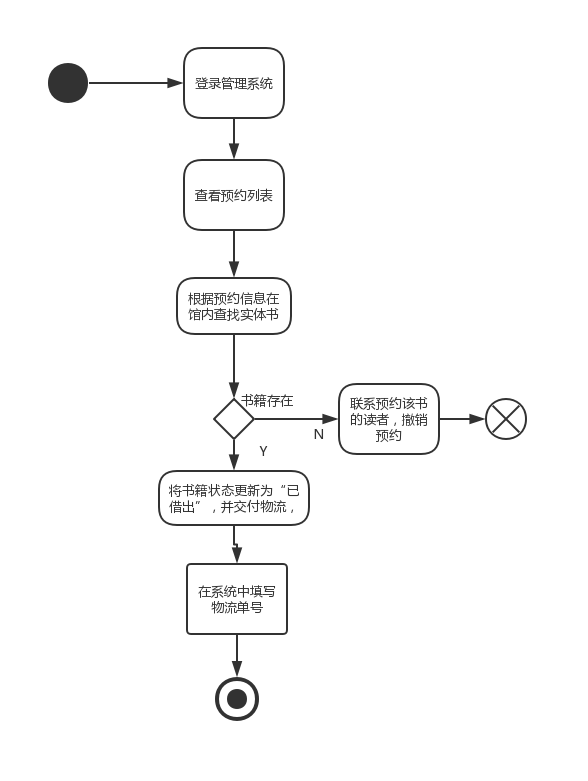
\includegraphics[width=0.45\textwidth]{./Chapters/images/activity_handle_borrow.png}}
    \subfigure[处理还书活动图]{
    \label{处理还书活动图}
    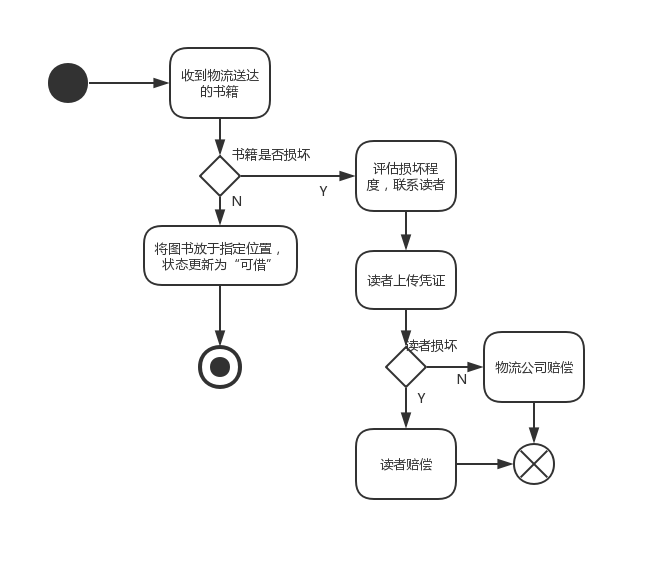
\includegraphics[width=0.45\textwidth]{./Chapters/images/activity_handle_back.png}}
    \caption{处理借还书活动图}
    \label{处理借还书活动图}
\end{figure}
\subsection{业务规则}
\begin{itemize}
    \item 借还书时间规定,书籍的借出时间为管理员修改书籍为"已借出"的具体时间,归还时间为管理员修改书籍状态为"已归还",或用户亲自到馆归还的具体时间。其中,物流配送时间算借书时间内。以四川大学图书馆为例,用户借书期限为30天,如果某用户通过本系统异地借阅书籍,实际取得书籍的时间是小于30天的。    
\end{itemize}
\subsection{非功能性需求}
\begin{itemize}
    \item 系统稳定性。由于系统具有展示、预约,还书、记录物流的功能。用户会在页面间来回跳转,点击。应该设计好页面的路由规则,预约请求的幂等性,维护预约事件列表,处理好事件循环,保证系统在网络异常或暴力操作时的数据准确性和系统稳定性。
    \item 系统安全性。由于本系统基于web端访问,应处理好XSS、CSRF、SSRF、DDoS等安全攻击,系统采用登录保护,没有借书卡的用户不允许登录,同时进行token校验,refer验证等方式,一定程度上保护了个人隐私,提高用户的信息安全性。
    \item 交互友好性。本系统为用户提供友好美观的图文操作页面,采用流式布局,分析用户操作流程,优化界面布局和操作步骤,提供优质的用户体验。同时,在书籍即将超期时推送消息,提醒用户进行及时还书。
\end{itemize}

%!TEX root = ../MainBody.tex

% 第三章
\chapter{系统设计}% 使用\cite{}命令引用数据库中文献
\section{相关概念}
\subsection{TypeScript}
TypeScript是一种由微软开发的自由和开源的编程语言。它是JavaScript的一个严格超集,并添加了可选的静态类型和基于类的面向对象编程的首席架构师以及Delphi和Turbo Pascal的创始人安德斯·海尔斯伯格参与了TypeScript的开发。TypeScript支持为现存JavaScript库添加类型信息的定义文件,方便其他程序像使用静态类型的值一样使用现有库中的值。当前有第三方提供常用库如MongoDB、Node.js和D3.js等的定义文件。TypeScript是一种给JavaScript添加特性的语言扩展。增加的功能包括:类型批注和编译时类型检查、类型推断、类型擦除、接口、枚举、泛型编程、Mixin、命名空间、元组、await等。运行于任何平台上的任何网页浏览器都可以运行TypeScript:由于它仅仅是被编译为标准的JavaScript,一个脚本不仅可以被预编译为文件,也能通过为TypeScript包含JavaScript编译器进行实时编译。
\subsection{React}
React是一个高效而且灵活的用来构建用户界面的框架。具有声明式、组件化的特点。React视图通常采用包含以自定义HTML标记规定的其他组件的组件渲染。React为程序员提供了一种子组件不能直接影响父组件("data flows down")的模型,数据改变时对HTML文档的有效更新,和现代单页应用中组件之间干净的分离。

它由Facebook、Instagram和一个由个人开发者和企业组成的社群维护。根据JavaScript分析服务Libscore,React当前正在被Netflix、Imgur、Bleacher Report、Feedly、Airbnb、SeatGeek、HelloSign等很多网站的主页使用。
\subsection{Webpack}
Webpack 是一个成熟的开源前端模块化打包工具。Webpack 提供了前端开发缺乏的模块化开发方式,将各种静态资源视为模块,并从它生成优化过的代码

Webpack可以从客户端、或是更改 webpack.config.js配置文件来设置各项功能。

本质上,*webpack* 是一个现代 JavaScript 应用程序的*静态模块打包器(module bundler)*。当 webpack 处理应用程序时,它会递归地构建一个*依赖关系图(dependency graph)*,其中包含应用程序需要的每个模块,然后将所有这些模块打包成一个或多个 *bundle*。

要使用 Webpack 前须先安装 Node.js。Webpack 其中一个特性是使用加载器(loader)来将不同类型资源转化成对应模块。开发者可以自定义加载器的顺序、格式来因应项目的需求。
\subsection{MongoDB}
MongoDB是一种面向文档的数据库管理系统,由C++撰写而成,提供高性能,高可用性和自动扩展。MongoDB中的一条记录就是一个文档,是一个数据结构,由字段和值对组成。MongoDB文档与JSON对象类似。字段的值有可能包括其它文档、数组以及文档数组。MongoDB提供高性能的数据持久化,支持丰富的查询语言,具有高可用性和水平扩展能力且支持多存储引擎。
\section{功能设计}
\subsection{读者功能模块}
\begin{itemize}
    \item 读者登录模块。用户第一次访问系统时进入的模块,读者的账号密码输入成功之后,才能进入主界面,即浏览借阅模块。
    \item 浏览借阅模块。功能点为展示图书基本信息、可借数量和提供预约借书操作,该模块展示一个馆藏图书列表,每一个列表项用卡片表示,卡片中包含书籍的基本信息、馆藏状态、是否可借等信息,并且有一个预约按钮,当书籍为可借数量大于1时,按钮可点击。
    \item 在借图书模块。该模块功能点包括展示预约图书列表和待还图书列表。预约图书列表的每一项展示预约书籍的基本信息,且有一个取消借阅按钮,点击可取消借阅。待还图书列表的每一项展示该书籍的基本信息和实际借阅日期,且有一个还书按钮,点击该按钮可提交还书申请,弹出确认框,填写物流单号,点击确认框的"确认"按钮提交还书申请。
    \item 个人信息模块。该模块的功能点为展示读者账号信息,物流地址增删改,展示收藏列表等。
\end{itemize}
\begin{figure}[H] %H为当前位置,!htb为忽略美学标准,htbp为浮动图形
    \centering %图片居中
    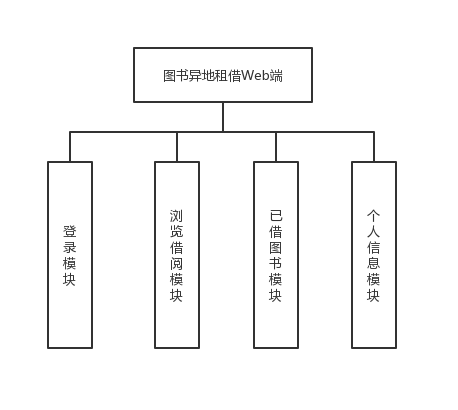
\includegraphics[width=0.7\textwidth]{./Chapters/images/reader_module.png} %插入图片,[]中设置图片大小,{}中是图片文件名
    \caption{读者模块} %最终文档中希望显示的图片标题
    \label{读者模块} %用于文内引用的标签
\end{figure}

\subsection{管理员功能模块}
\begin{itemize}
   \item 登录模块:管理员访问系统时进入的模块,系统验证成功之后,方可进入主界面。
   \item  预约列表模块:该模块功能点为展示读者预约的图书列表和预约状态修改,列表每一项包含图书名称、借书条码号、是否已借出的按钮。在管理员将书籍交付物流之后,点击该书籍所在项的按钮,弹出确认框,管理员在确认框中填写物流单号,点击确认提交信息。
   \item 待还列表模块:该模块功能点为展示通过本系统借阅的书籍、发出还书请求,但还在物流配送途中,并未被图书馆签收的书籍列表。每一项包含书籍的基本信息、借书条码号、应还日期等信息。
   \item 异常书籍模块:功能点为展示借阅过程中出现异常的书籍列表,如遗失、损坏的书籍和修改书籍异常状态。列表每一行展示异常书籍的基本信息、异常类别和异常状态修改按钮,点击该按钮可将异常书籍标记为正常,下次访问该模块时,上次标记为正常的书籍将不会展示在该模块的列表中。   
\end{itemize}

\begin{figure}[H]
    \centering
    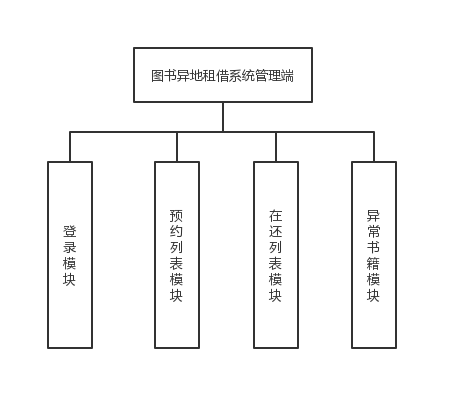
\includegraphics[width=0.7\textwidth]{./Chapters/images/admin_module.png} %插入图片,[]中设置图片大小,{}中是图片文件名
    \caption{管理员模块} %最终文档中希望显示的图片标题
    \label{管理员模块} %用于文内引用的标签   
\end{figure}
\section{架构设计}
\begin{figure}[H]
    \centering
    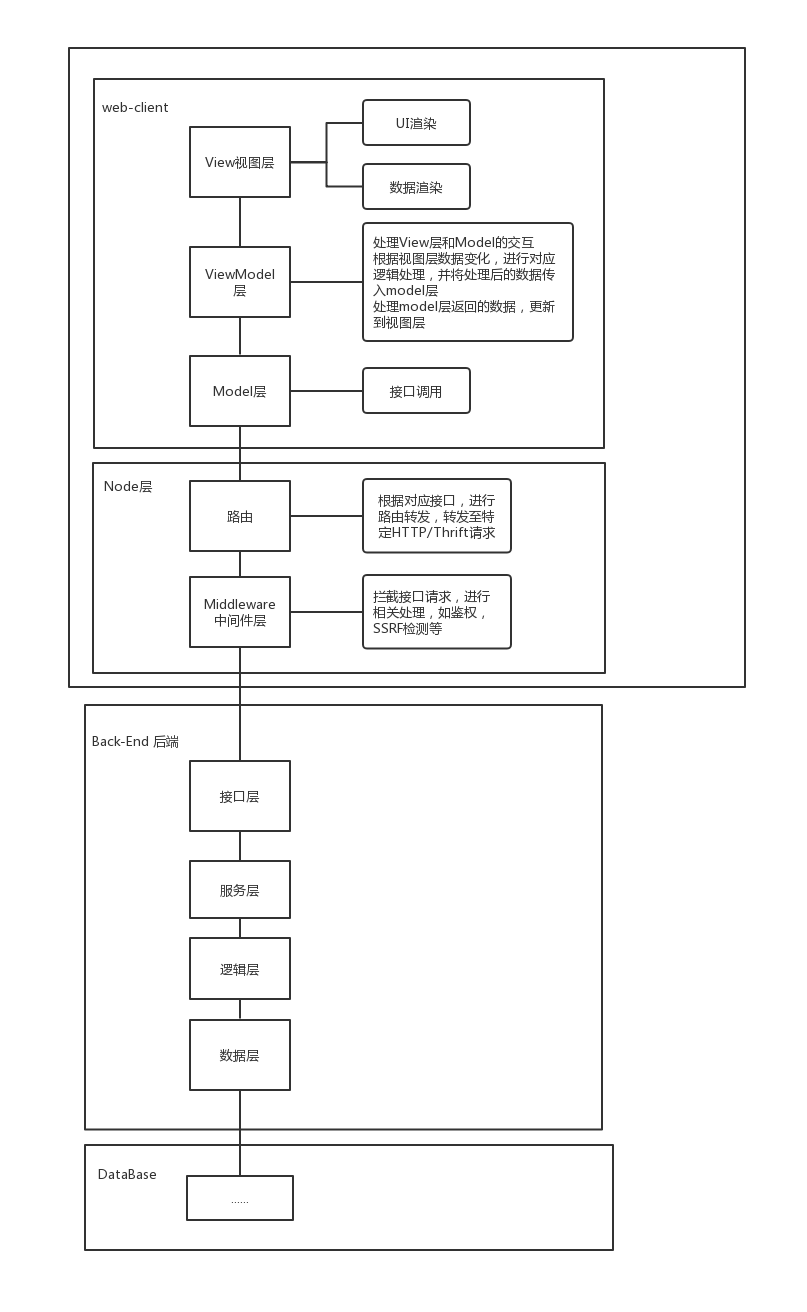
\includegraphics[width=0.7\textwidth]{./Chapters/images/system_structure.png} %插入图片,[]中设置图片大小,{}中是图片文件名
    \caption{系统架构图} %最终文档中希望显示的图片标题
    \label{系统架构图} %用于文内引用的标签   
\end{figure}
\subsection{web客户端}
web客户端采用由MVC(Model-View-Controller)架构衍生而来的MVVM架构。作为十分常见的前端架构之一,在项目中具有非常广泛的应用。MVVM架构由View层(视图层)、ViewModel层(视图模型层)、Model层(模型层)三部分组成。

视图层,是屏幕展示视图的封装,是程序中处理数据展示的部分,用于可视化界面的展示和捕捉用户进行的各种交互操作。视图层不涉及业务逻辑,只是通过访问它所监视的视图模型,实现相应视图的更新。

视图模型层,用于处理所有和业务逻辑相关的代码,完全不涉及UI部分。当View层数据发生变化时,省去中间冗余的接口,而直接驱动UI的对应变化。视图模型层承载的内容为视图展现逻辑,视图层所需的数据由视图模型层进行逻辑转换得到,转换前的初始数据可能由服务器返回、数据库获取或用户输入,这种"未经格式化"的原始数据往往无法用于视图层直接展示,视图展现逻辑就是将这些原始数据经过一系列逻辑拆分转化,处理成可以用于屏幕展示的数据。视图模型层中的每个的方法代码所处理的功能具有单一性,且与外部不产生联系,使得代码更为健壮,易于维护。

模型层。实现对业务功能和应用状态的封装,可以将其理解为同时包含数据和行为的领域模型,通常情况下模型对象负责在数据库中获取、修改数据。模型起到定义若干模板额作用,不参与实际的业务逻辑,只是对模型层进行了一层抽象,将服务端返回的JSON对象中的字段一一 映射到事先定义好的数据模型中。在业务实现中,在Model层发起具体的HTTP请求,请求经过Node层拦截处理,返回响应数据。模型层的作用实际上是实现服务端数据在web客户端的映射,这个映射过程就是web端底层发起网络请求,并获取到数据的过程,映射的结果是一个单纯的数据结构,可以用struct表征。

MVVM的核心思想是“数据模型数据为绑定”,数据绑定的关键在于视图层和视图模型层之间的信息传递,层与层之间需要进行通信交流。在MVVM架构中,这一问题是通过"观察者模式"的具体应用——响应式编程实现的。

如何实现所谓的响应式编程?在WPF中官方提供了Data Binding技术,mac系统中也有类似的Cocoa Binding框架,GitHub上也出现了RAC(ReactiveCococa)和RxSwift等第三方开源框架。
在RAC的思维中,视图层的一切均为在变化的数据流,比如用户在输入框上不断输入的文字、被点击的按钮、旋转缩放的视图等等,这些就像是一个“水龙头”,当变化产生的时候,水龙头就会出水,向下传递变化,对这个变化感兴趣的人,即订阅者(subscriber),就可以在这个水龙头上套一个"水管"。通过提供统一的消息传递机制,位于下游的接收者能够及时收到变化,拿到这个变化的具体信息,并进行相关处理。具体来说,视图层哥视图模型层互为订阅者和传播者,双向绑定数据变化,视图层更新视图,视图模型层更新数据,并将更新的数据下发至模型层。
\subsection{Node层}
为了更好的实现前后端分离,在项目中引入node作为中间层,降低耦合度,处理大量重复逻辑。node层的主要作用是作为中间层,拦截和处理网络请求,并对请求头或响应数据进行业务处理。如在request请求头中加入设置允许跨域、加入校验token等,重定向后端返回的特殊响应code、SSRF、CSRF等安全拦截、通过映射解决前后端字段参数或字段类型不统一、日志上报等。对于web客户端来说,在浏览器上做运算、做分组、以及一系列操作是一定会影响性能的、尤其数据量很大的情况,可能出现首屏加载时间长、响应速度变慢以及页面卡顿等问题,用户体验因此大打折扣。对于开发人员来说,需要处理大量本可复用的逻辑,增加代码量和开发时长,同时项目质量却下降。而使用node中间层,则相当于把众多影响性能的代码放入其中,不影响浏览器的性能,同时替后端分担一些简单的数据逻辑、处理网络请求维度的公共逻辑,使得前后端的分离更为明确和彻底。

本项目中主要使用Koa框架来实现node中间层,主要作用为转发网络请求的数据,串接前后端;路由转发,修改请求头、简单处理相应数据;处理网络请求的特殊code,根据实现约定好的code规则进行逻辑映射;拦截SSRF/CSRF等前端安全攻击;用户和不同网络请求的权限控制;日志上报等。
\begin{figure}[H]
    \centering
    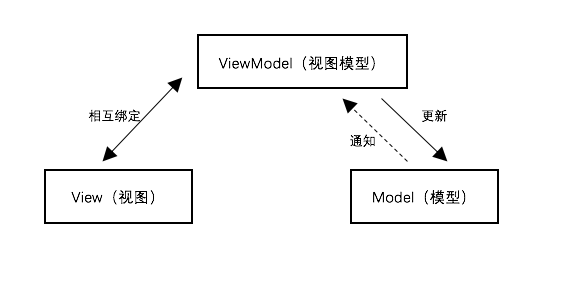
\includegraphics[width=0.7\textwidth]{./Chapters/images/mvvm.png} %插入图片,[]中设置图片大小,{}中是图片文件名
    \caption{MVVM模型} %最终文档中希望显示的图片标题
    \label{MVVM模型} %用于文内引用的标签   
\end{figure}
\section{时序图}
\begin{figure}[H]
    \centering
    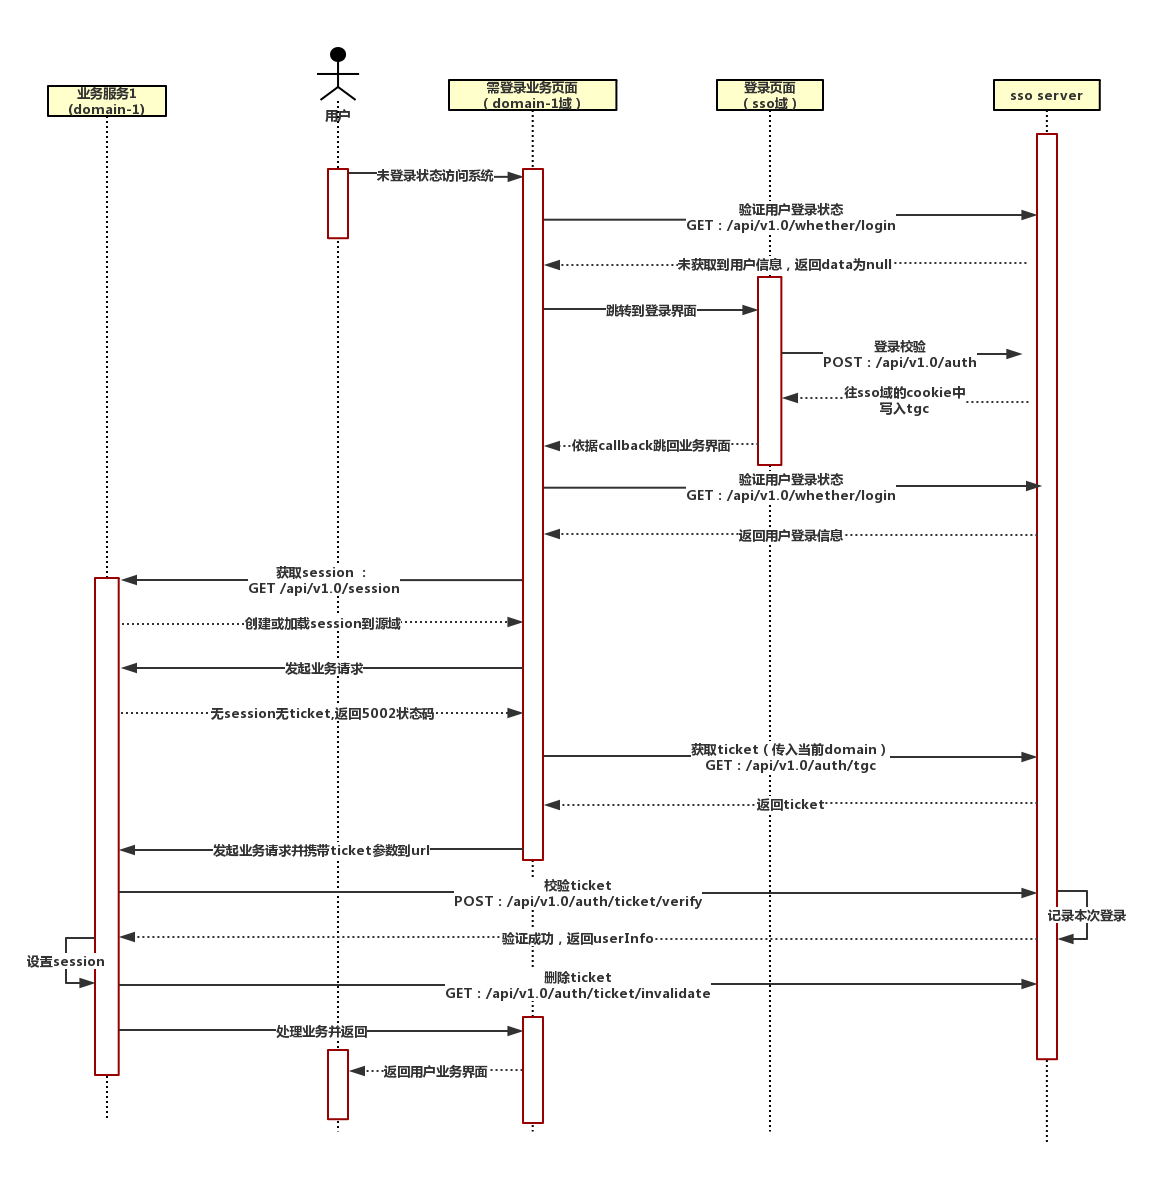
\includegraphics[width=0.7\textwidth]{./Chapters/images/time_gram_login.png} %插入图片,[]中设置图片大小,{}中是图片文件名
    \caption{登录时序图} %最终文档中希望显示的图片标题
    \label{登录时序图} %用于文内引用的标签   
\end{figure}
\begin{figure}[H]
    \centering
    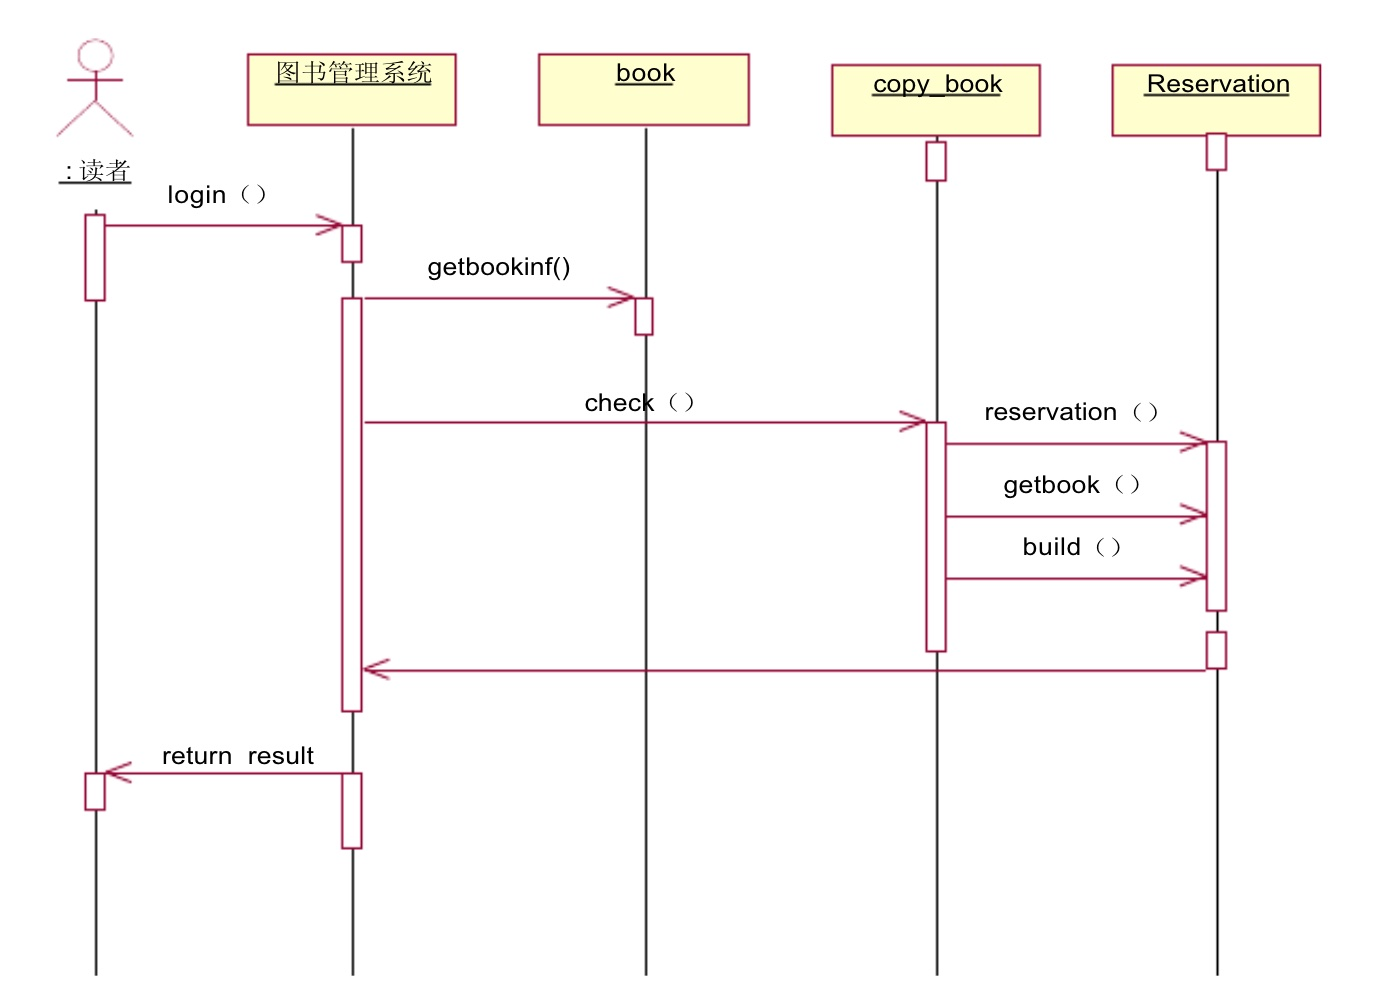
\includegraphics[width=0.7\textwidth]{./Chapters/images/time_diagram_borrow.png} %插入图片,[]中设置图片大小,{}中是图片文件名
    \caption{借书时序图} %最终文档中希望显示的图片标题
    \label{借书时序图} %用于文内引用的标签   
\end{figure}
\begin{figure}[H]
    \centering
    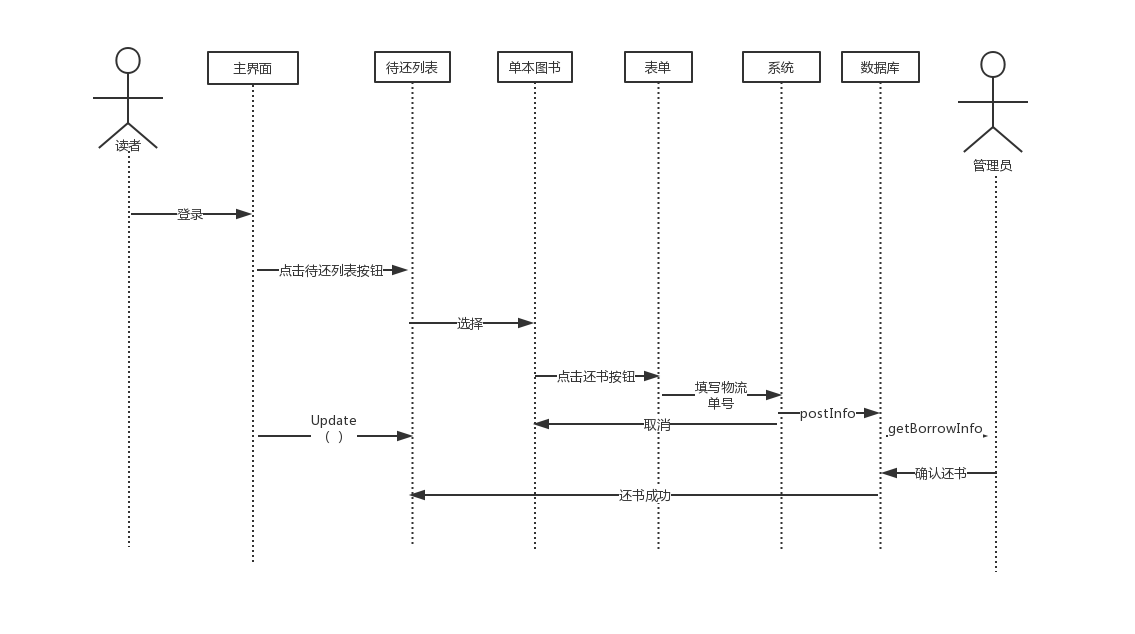
\includegraphics[width=0.7\textwidth]{./Chapters/images/time_diagram_back.png} %插入图片,[]中设置图片大小,{}中是图片文件名
    \caption{还书时序图} %最终文档中希望显示的图片标题
    \label{还书时序图} %用于文内引用的标签   
\end{figure}
\section{类图}
\begin{itemize}
    \item Reader类是读者类,包含若干属性和操作。属性有读者ID(userId)、姓名(userName)、地址(address[])、预约书目(borrowed[])、待还书目(toReturned[]),主要操作有预约借书(borrowBook)、还书(returnBook)等
    \item Admin是管理员类,包含管理员编号(adminId)、管理员姓名(adminName),操作主要有处理借书单据(handleBookBorrow)和处理还书单据(handleBookReturn)等。
    \item BookInfo是记录图书信息的类,属性包括书籍ISBN号、书籍名称、作者、出版社、内容简介等
    \item BookBorrowInfo是书籍借阅信息类,包含书籍条码号、可借数量、馆藏数量、馆藏位置等属性。
    \item Borrow是具体某书的借阅信息,包括书籍条码号、借书物流单号、还书物流单号、借阅时间等属性。
\end{itemize}
\begin{figure}[H]
    \centering
    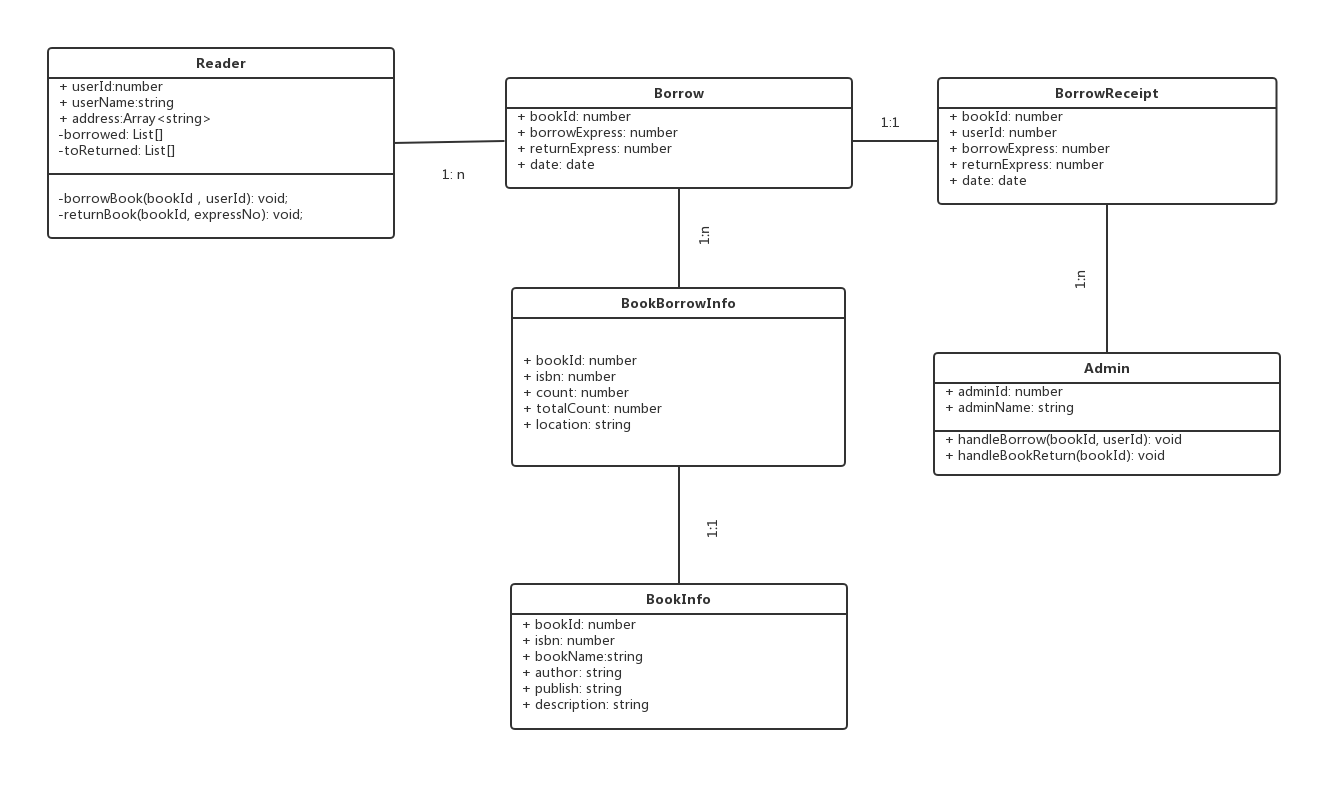
\includegraphics[width=0.7\textwidth]{./Chapters/images/class_diagram.png} %插入图片,[]中设置图片大小,{}中是图片文件名
    \caption{类图} %最终文档中希望显示的图片标题
    \label{类图} %用于文内引用的标签   
\end{figure}
% \section{数据库设计}
% \subsection{实体图}
% 读者:读者属性有账号、姓名、密码、地址、已借书籍信息、预约书籍信息。实体图如图所示:
% 图书:图书属性有图书编号、书名、作者、出版者、出版信息、总数量、可借数量、内容摘要。实体图如图所示:
% \begin{figure}[H]
%     \centering  %图片全局居中
%     \subfigure[读者实体图]{
%     \label{读者实体图}
%     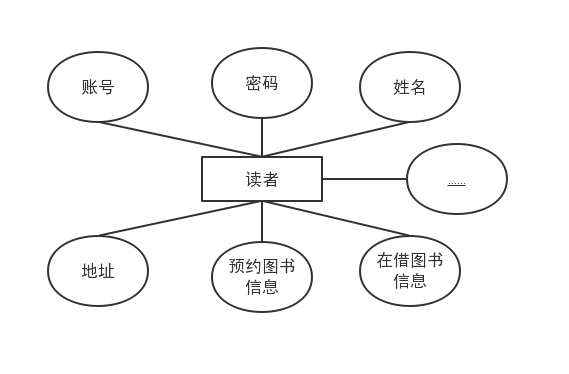
\includegraphics[width=0.45\textwidth]{./Chapters/images/reader_entity.png}}
%     \subfigure[图书实体图]{
%     \label{图书实体图}
%     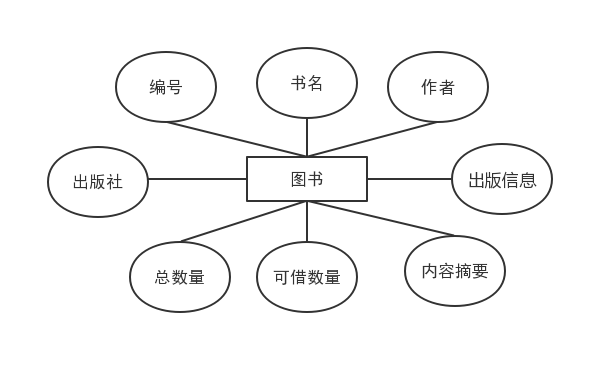
\includegraphics[width=0.45\textwidth]{./Chapters/images/book_entity.png}}
%     \caption{实体图}
%     \label{实体图}
% \end{figure}
% \begin{figure}[H]
%     \centering
%     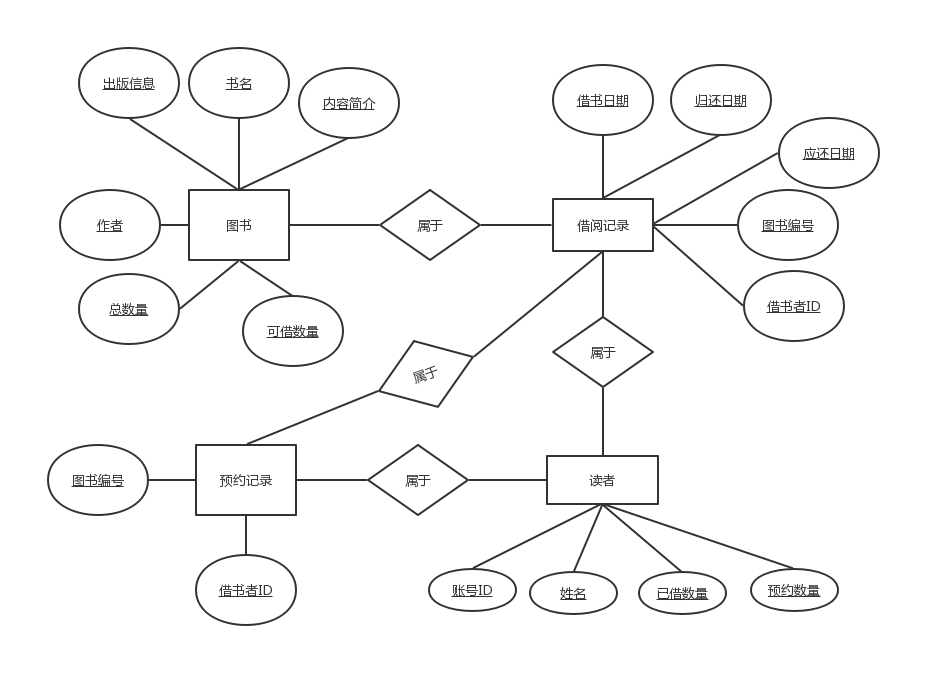
\includegraphics[width=0.7\textwidth]{./Chapters/images/ER.png} %插入图片,[]中设置图片大小,{}中是图片文件名
%     \caption{E-R图} %最终文档中希望显示的图片标题
%     \label{E-R图} %用于文内引用的标签   
% \end{figure}
\section{接口设计}
web客户端层的网络请求基于axios第三方api自定义,基础配置为:允许跨域;baseURL为'http://localhost:2222/apihttp://localhost:2222/api/';超时时间设置为10000毫秒;返回响应数据类型为json; 返回响应数据为UTF-8。

\textbf{获取图书列表}

url: 'api/book/list'

method: 'GET'

\begin{tabular}{lllll|}
    \hline
    Request URL参数& 类型& 是否必填& 默认值 & 备注\\
    pageNo & number & 是& 1& 页码\\
    pageSize & number & 是& 20& 页数\\
    keyword& string& 否& -& 关键词\\
    \hline
\end{tabular}

注:除了params对象外,还可传入自定义请求头,可包含登录token,CSRF校验token等信息。

\begin{tabular}{lllll}
    \hline
    Response data对象& 类型& 是否非空& 默认值 & 备注\\
    
    bookNo & number & 是& 1& 页码\\
    
    name & string& 是& 20& 页数\\
    
    author& string& 是& -& 作者\\
   
    press& string& 否& -& 出版社\\
    
    count& number& 是& -& 可借数量\\
    totalCount& number& 是& -& 馆藏总数量\\
    publishInfo& string& 否& -& 出版信息\\
    description& string& 是& -& 简介\\
    \hline
\end{tabular}

\textbf{提交借书请求:}

url: '/api/book/borrow';

method: 'POST';

\begin{tabular}{lllll}
    \hline
    Request body对象& 类型& 是否必填& 默认值 & 备注\\
    bookNo & number& 是& -& 图书编号\\
    userNo & number& 是& -& 读者编号\\
    createdTime& date& 否& Date.now()& 借书日期\\
    \hline
\end{tabular}

请求成功,response code返回200。

\textbf{获取预约列表:}

url: '/api/book/list/borrow';

method: 'GET'

\begin{tabular}{lllll}
    \hline
    Request URL参数& 类型& 是否必填& 默认值 & 备注\\
    
    pageNo & number & 是& 1& 页码\\
    
    pageSize & number & 是& 20& 页数\\
    \hline
\end{tabular}

\begin{tabular}{lllll}
    \hline
    Response data对象& 类型& 是否非空& 默认值 & 备注\\
    
    bookNo & number & 是& 1& 图书编号\\
    
    bookName & number& 是& 20& 图书名称\\
    
    expressNo& string& 是& -& 物流单号\\
    \hline
\end{tabular}

\textbf{获取个人信息:}

url: '/api/user/info';

method: 'GET'

\begin{tabular}{|l|l|l|l|l|}
    \hline
    Request URL参数& 类型& 是否必填& 默认值 & 备注\\
    \hline
    id & number & 是& -& 读者ID\\
    \hline
    name & number & 是& -& 读者姓名\\
    \hline
    address & string[] & 否& -& 收货地址\\
    \hline
\end{tabular}

如果上述请求成功,返回response的code为200,如果请求失败,返回下列code之一:

404:请求未找到

500:服务器内部错误

502:访问服务器被拒绝,响应无效

10002:用户鉴权失败

10005:字段类型错误

10012:其他原因,借书失败

\section{界面及交互设计}
\subsection{登录模块}
登录界面中输入借书账号和密码,验证通过则进入主界面,对于验证失败的情况:账号不存在,弹出toast提示"账号不存在,请前往图书馆申请注册借书卡,凭借书卡账号密码登录";账号密码填写错误,系统弹出提示"账号或密码填写错误"。用户点击下方注册按钮,则弹出modal提示"请前往图书馆注册借书卡,凭借借书卡账号密码登录"。
\begin{table}[ht]
    \centering
    \begin{tabular*}{\textwidth}{p{0.3\textwidth}p{0.7\textwidth}}
        \hline
        用户行为  & 系统显示 \\
        \hline
        进入登录界面 & 显示登录界面 \\
        输入账号密码 & 输入框显示用户刚刚输入的内容 \\
        点击登录按钮,登录失败 & toast显示提示文案:"账号不存在"或"账号或密码输入有误"\\
        点击登录按钮,登录成功 & toast显示"登录成功",显示加载条,跳转到主界面 \\
        \hline
    \end{tabular*}
    \begin{tabular*}{\textwidth}{p{0.3\textwidth}p{0.7\textwidth}}
        \hline
        窗口/对话框  & GUI组件 \\
        \hline
        登录界面 & 登录图标,登录表单:账号输入框,密码输入框,登录按钮 \\
        \hline
    \end{tabular*}
\end{table}
\subsection{主界面}
% \begin{figure}[H]
%     \centering
%     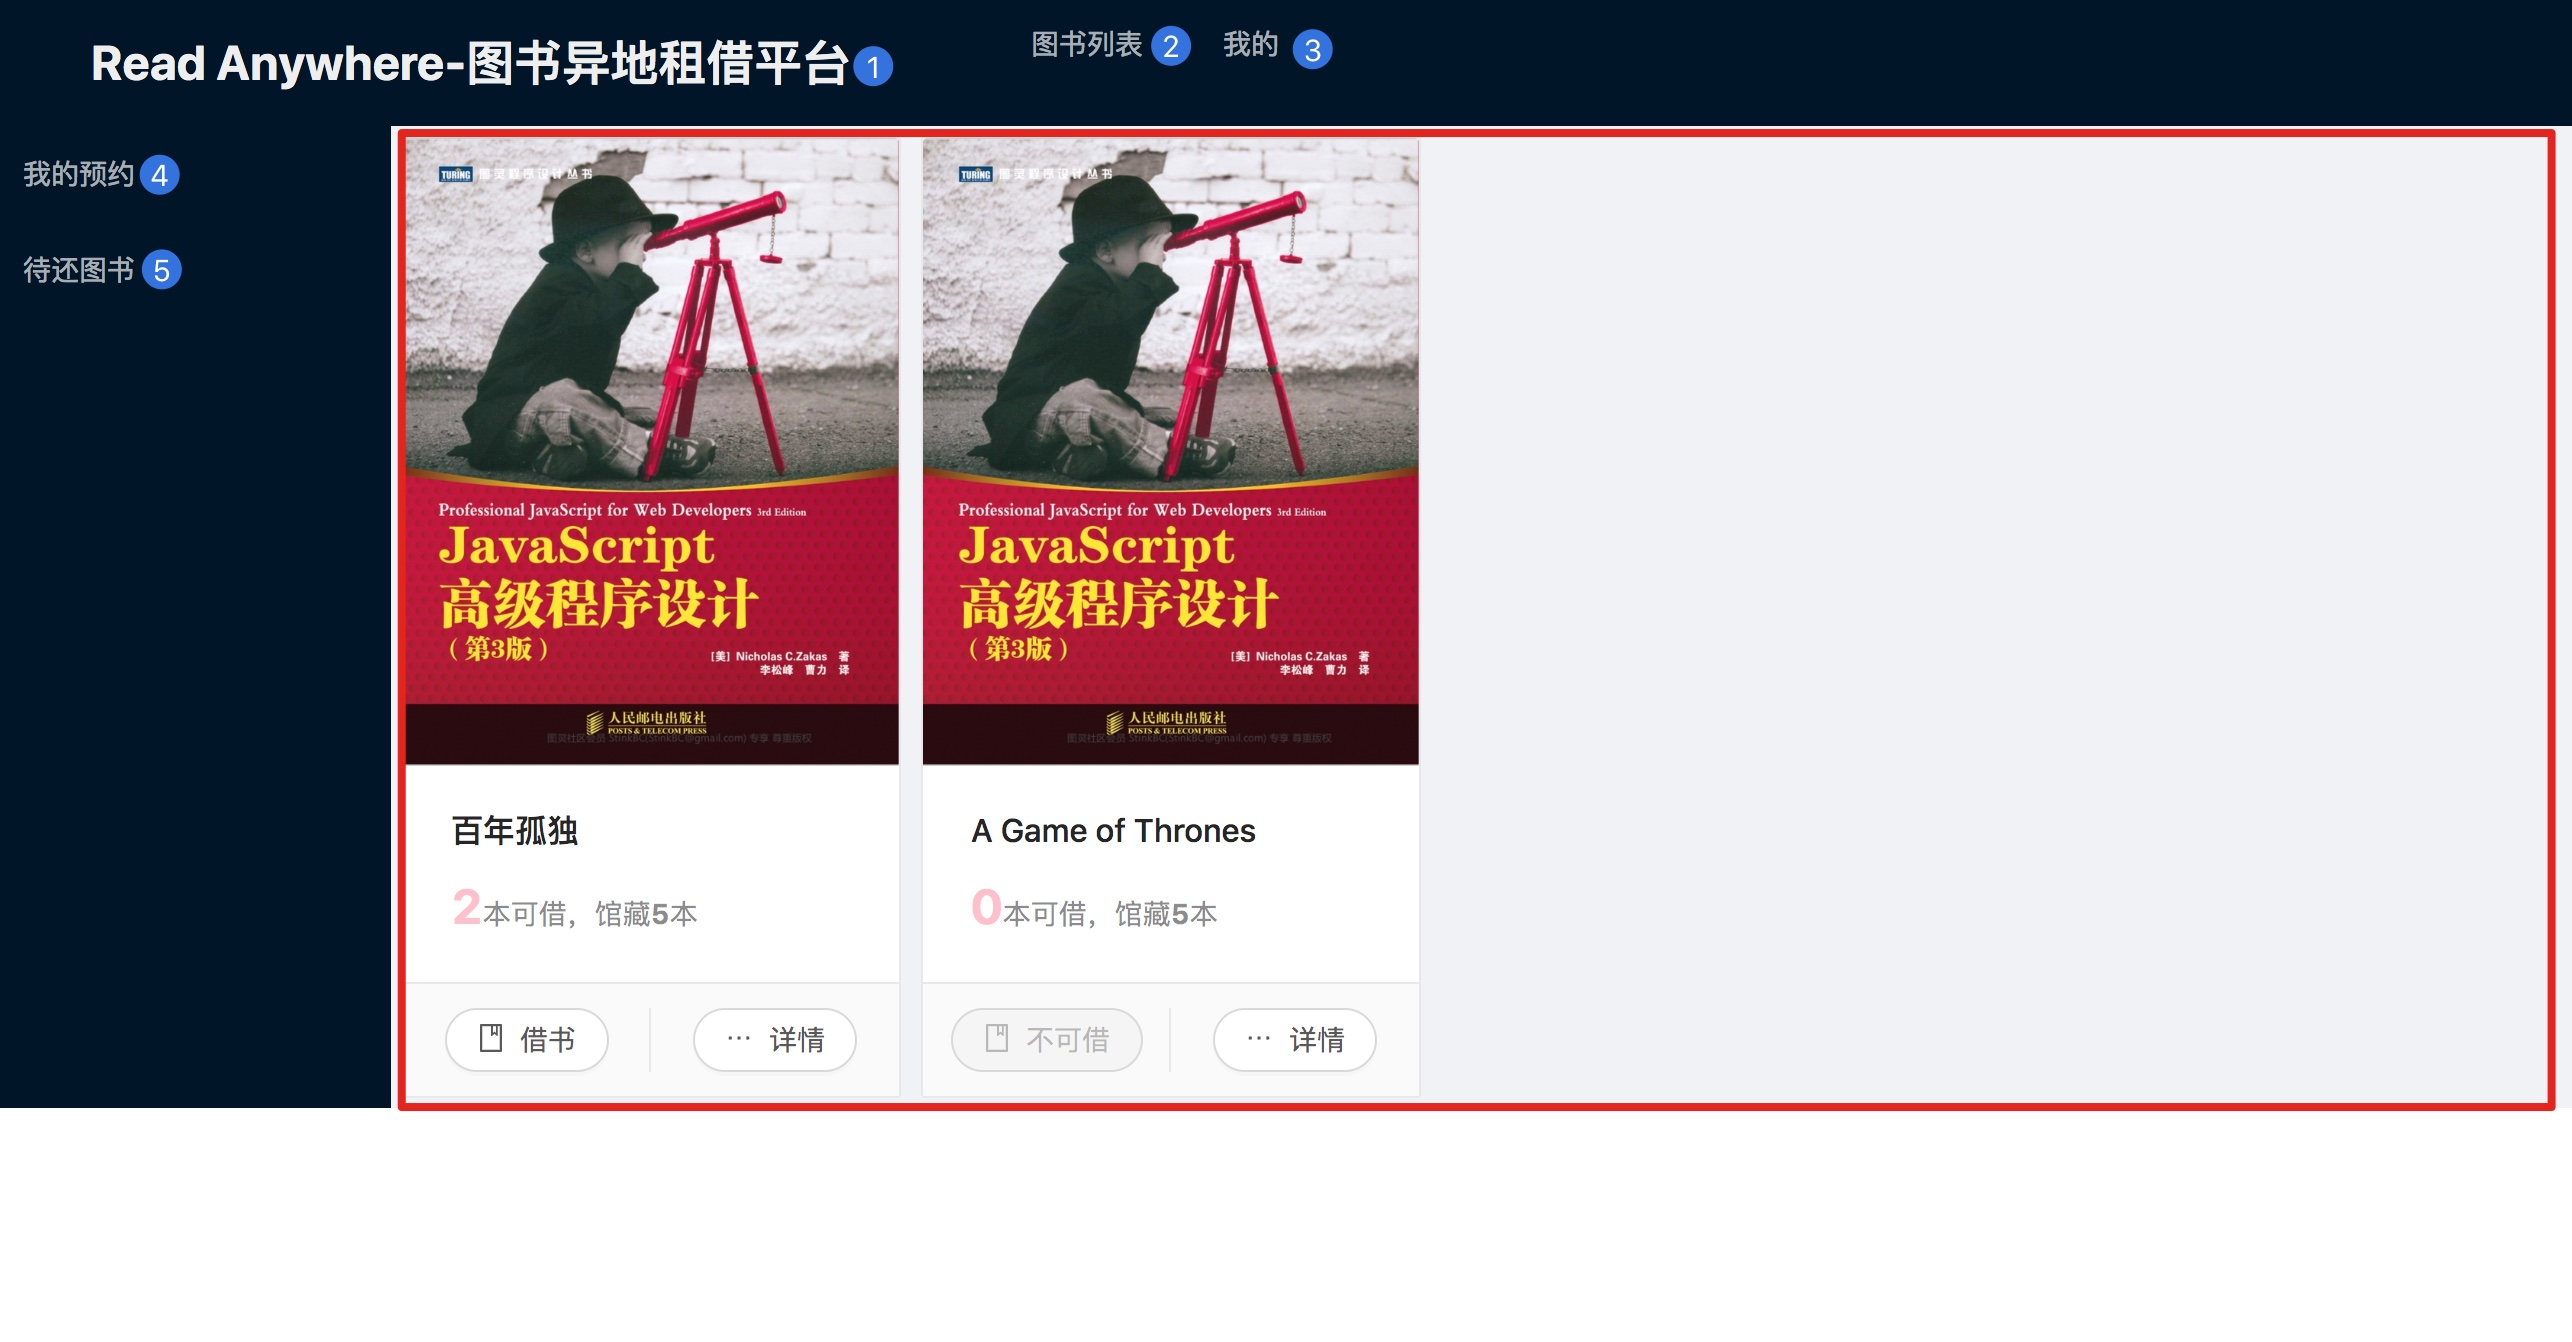
\includegraphics[width=\textwidth]{./Chapters/images/mainUI.png} %插入图片,[]中设置图片大小,{}中是图片文件名
%     \caption{界面设计-主界面} %最终文档中希望显示的图片标题
%     \label{界面设计-主界面} %用于文内引用的标签   
% \end{figure}
% 上图红色方框框住的部分为内容区,图中序号标注参考如下:
% \begin{enumerate}
%     \item 显示平台名称,字体格式为H1
%     \item 内容区默认显示的内容与点击“图书列表”导航按钮的内容一致,显示图书列表,每个列表项包含图书的封面、书名、馆藏数量、可借数量、简介等信息,馆藏数量大于0时,借书按钮可点击,否则不可点击。点击详情按钮,按钮上方弹出气泡,显示书籍简介信息
%     \item 点击“我的”导航按钮,内容区显示“我的”模块的信息
%     \item 点击“我的预约”菜单项,内容区显示预约列表
%     \item 点击“待还图书”菜单项,内容区显示待还图书列表
% \end{enumerate}
% 主界面的主框架包含上方导航栏、左侧菜单栏和底部信息栏。剩余的中部和右侧为内容区。内容区作为容器,根据导航栏或菜单栏的具体项显示对应数据。导航栏有"书籍列表"和"我的"两个Tab,页面的内容区默认显示"书籍列表"Tab下的内容。点击导航栏的"我的"Tab,内容区显示个人信息。进入主界面时会有网络请求,请求第一页的列表数据。
登录成功后系统会跳转到主界面,进入主界面时浏览器会发起网络请求,请求书籍列表数据。在网络请求成功之前界面一直显示Loading动画,数据请求成功后动画消失:
\begin{table}[ht]
    \centering
    \begin{tabular*}{\textwidth}{p{0.3\textwidth}p{0.7\textwidth}}
        \hline
        用户行为 & 系统显示\\
        \hline
        进入主界面 & 进入主界面时内容区显示加载圈,加载成功之后,内容区默认显示图书列表模块数据\\
        点击“图片列表”导航按钮 & 内容区显示图片列表信息 \\
        点击“我的”导航按钮 & 内容区显示“我的”模块的信息 \\
        点击“我的预约” & 内容区显示“预约列表”信息 \\
        点击“待还图书” & 内容区显示“待还列表”信息 \\
        点击“退出”按钮 & 退出系统,跳转至登录界面 \\
        \hline
    \end{tabular*}
    \begin{tabular*}{\textwidth}{p{0.3\textwidth}p{0.7\textwidth}}
        \hline
        窗口/对话框  & GUI组件 \\
        \hline
        导航栏 & 平台名称;“图书列表”按钮;“我的”按钮,用户姓名,退出按钮\\
        菜单栏 & “我的预约”菜单项;“待还图书”菜单项 \\
        内容区 & 根据用户点击的导航按钮或菜单项,显示对应模块的内容,默认显示图书列表模块的内容 \\
        \hline
    \end{tabular*}
\end{table}

用户点击导航栏或菜单项时,系统会对应加载数据,显示到内容区,如加载图书列表数据时:
\begin{enumerate}
    \item 请求成功且有数据,则将数据传入列表,展示到页面。书籍列表包含包含若干个卡片,每个卡片展示单本书籍的封面、条码号、作者、书名、简介、馆藏数量、可借数量,如果可借数量大于一本,则借书按钮是可点击的,否则按钮置灰,不可点击。
    \item 请求成功,但无数据,内容区展示"暂无数据"样式。
    \item 请求失败,弹出toast提示"请求失败,请重试",内容区展示"暂无数据"样式。
\end{enumerate}
用户点击导航栏的其他Tab,会发送网络请求请求对应数据,与上述"请求书籍列表"的逻辑流程类似。同时列表为分页懒加载,每页的数量为20条,用户点击对应页码按钮,请求和展示对应页码的数据。布局为弹性布局,根据窗口大小实现比例自适应。
\subsection{“图片列表”模块}
“图片列表”模块,显示书籍的信息,提供预约借书按钮和取消预约按钮,取消预约操作也可在预约列表中进行。
\begin{table}[ht]
    \centering
    \begin{tabular*}{\textwidth}{p{0.3\textwidth}p{0.7\textwidth}}
        \hline
        用户行为 & 系统显示\\
        \hline
        书籍可借数量大于1时,点击“借书”按钮 & 弹出二次确认框,确认后系统显示加载圈,请求结束后加载圈消失 \\
        书籍可借数量为0,点击“借书”按钮 & 按钮不可点击 \\
        点击“取消预约”按钮& 弹出二次确认框,确认后系统显示加载圈,请求结束后加载圈消失 \\
        点击“详情”按钮 & “详情”按钮上方显示气泡,气泡中显示书籍简介信息,再次点击或点击其他按钮,气泡消失 \\
        \hline
    \end{tabular*}
    \begin{tabular*}{\textwidth}{p{0.3\textwidth}p{0.7\textwidth}}
        \hline
        窗口/对话框  & GUI组件 \\
        \hline
        图书列表项 & 书籍封面;书名;可借数量;馆藏数量;预约按钮;详情按钮\\
        点击预约按钮后弹出的确认框 & 文案为:“确认预约本书?”,下方有确认按钮和取消按钮 \\
        书籍可借数量为0状态下的“借书”按钮 & 按钮置灰,不可点击\\
        点击详情按钮弹出的气泡 & 气泡在详情按钮正上方显示,高度不超过200px \\
        \hline
    \end{tabular*}
\end{table}
\newpage
\subsection{"我的"模块}
“我的”模块中,显示读者个人信息、收货地址,同时提供跳转至预约列表、待还列表的按钮。
\begin{table}[ht]
    \centering
    \begin{tabular*}{\textwidth}{p{0.3\textwidth}p{0.7\textwidth}}
        \hline
        用户行为 & 系统显示\\
        \hline
        点击“我的预约”列表项 & 跳转至预约列表,内容区显示预约列表数据\\
        点击“待还图书”列表项 & 跳转至待还列表,内容区显示待还图书数据 \\
        点击“物流地址”列表项& 列表项下方展开显示物流信息 \\
        \hline
    \end{tabular*}
    \begin{tabular*}{\textwidth}{p{0.3\textwidth}p{0.7\textwidth}}
        \hline
        窗口/对话框  & GUI组件 \\
        \hline
        “我的”界面 & 用户姓名;账号ID;“待还图书”列表项;“我的预约”列表项;“物流地址”列表项\\
        “物流地址”列表项 & 该列表项为一个折叠面板,点击展开,显示物流信息列表,包含列表项、新增地址按钮,每个列表项包含:联系人手机号;详细地址,编辑按钮,删除按钮;再次点击折叠面板收起 \\
        \hline
    \end{tabular*}
\end{table}
\newpage
\subsection{“我的预约”模块}
\begin{table}[ht]
    \centering
    \begin{tabular*}{\textwidth}{p{0.3\textwidth}p{0.7\textwidth}}
        \hline
        用户行为 & 系统显示\\
        \hline
        点击“取消预约” & 弹出二次确认框,确认框文案为:“确认取消预约?”\\
        \hline
    \end{tabular*}
    \begin{tabular*}{\textwidth}{p{0.3\textwidth}p{0.7\textwidth}}
        \hline
        窗口/对话框  & GUI组件 \\
        \hline
        预约列表项 & 书籍名称;预约日期;取消预约按钮\\
        预约列表 & 展示20条列表项,列表下方有分页按钮\\
        \hline
    \end{tabular*}
\end{table}
点击二次确认框之后,系统会显示加载圈,请求结束后加载圈消失,不同请求结果对应样式:
\begin{enumerate}
   \item 请求成功,弹出toast"请求成功",该列表项被删除,不再出现在预约列表中。
   \item 请求失败,弹出toast"请求失败,请重试",列表维持原样无变化。 
\end{enumerate}
\subsection{“待还图书”模块}
\begin{table}[ht]
    \centering
    \begin{tabular*}{\textwidth}{p{0.3\textwidth}p{0.7\textwidth}}
        \hline
        用户行为 & 系统显示\\
        \hline
        点击“我要还书” & 弹出表单框,填写物流信息\\
        点击表单框中的确认按钮 & 表单校验成功之后,显示加载圈,请求结束后加载圈消失,表单框消失\\
        点击表单框中的取消按钮 & 表单框消失。\\
        \hline
    \end{tabular*}
    \begin{tabular*}{\textwidth}{p{0.3\textwidth}p{0.7\textwidth}}
        \hline
        窗口/对话框  & GUI组件 \\
        \hline
        待还列表项(未填写过还书物流) & 书籍名称;借书日期;预约的物流单号;我要还书按钮\\
        待还列表项(已填写还书物流) & 书籍名称;借书日期;预约的物流单号;还书的物流单号;还书日期;修改物流按钮\\
        点击还书后弹出的表单框 & 表单中包含物流公司输入框;物流编号输入框;确认按钮;取消按钮。输入框内容均为空 \\
        点击修改物流后弹出的表单框 & 表单中包含物流公司输入框;物流编号输入框;确认按钮;取消按钮。输入框内容为上次填写的物流公司名和单号\\
        \hline
    \end{tabular*}
\end{table}
% 点击待还列表,路由跳转至对应页面,内容区展示一个懒加载的分页列表,页数20,每个列表项显示待还书籍的书名、条码号和"我要还书"按钮。点击"我要还书书",页面弹出modal框,在modal框的表单内填入物流信息,点击确认,发送对应网络请求。列表栏会显示对应物流单号和快递公司名称,右侧有一个编辑按钮,点击可修改物流信息。有物流单号时,不显示"我要换书"按钮。

% 收货地址栏中,包含收货地址信息,可新增、编辑、删除单条收货信息。每条收货地址信息的姓名、联系人号码、街道地址为必填。

% 点击退出按钮,弹出二次确认框,用户点击确认后,跳转至登录界面。







%!TEX root = ../MainBody.tex

% 第三章
\chapter{系统实现}% 使用\cite{}命令引用数据库中文献
\section{运行平台}
\begin{itemize}
    \item MacOS操作系统
    \item 开发工具:Visual Studio Code
    \item 浏览器:Chrome、Safari
    \item 编程语言:HTML5+SCSS+JavaScript(ECMAScript 6.0)
    \item 数据库:MongoDB
\end{itemize}
\section{功能界面}
\subsection{登录界面}
\subsection{主界面(图书列表界面)}
\section{代码}
\subsection{项目结构}
\begin{lstlisting}[numberstyle=\tiny,keywordstyle=\color{blue!70},
    commentstyle=\color{red!50!green!50!blue!50},frame=shadowbox,
    rulesepcolor=\color{red!20!green!20!blue!20},basicstyle=\ttfamily]
    |- dist // webpack 打包输出目录
    |- config    // webpack 构建配置目录  
    ​    |- tpl  
    ​        |- index.html 入口  
    ​    |- webpack.config.js    //  webpack 配置文件  
    |- node-modules  //  公共依赖  
    |- node-server  //  node 端  
    ​    |- main.js  
    ​    |- middleware // 中间件  
    ​    |- proxy.config.js // 前后端proxy配置   
    ​    |- route // 路由配置  
    |-- web-client 
    ​    |- common 公共资源,如图片、SVG等  
    ​    |- components   // 公共组件  
    ​    |- domain   // 处理网络请求   
    ​    |- model    // 页面与api请求之间的业务中间层  
    ​    |- styles   // 公共样式  
    ​    |- utils  //公共工具  
    ​    |- page  //页面 
    ​        |- A   // 页面A 
    ​            |- index.tsx  // 页面逻辑  
    ​            |- store.ts  // mobX 数据管理   
    ​        |- B  
    ​            |- index.tsx  
    ​            |- store.ts  
    |- package.json   
    |- .gitignore  
    |- README.md   
    |- stylelintrc.js // eslint 代码格式检查配置文件  
    |- tslint.json // tslint 代码格式检查配置文件   
    |- theme.js  // 修改antd主题色   
    |- tsconfig.json    
\end{lstlisting}
\subsection{关键代码}
界面框架及静态路由:

\begin{lstlisting}[numberstyle=\tiny,keywordstyle=\color{blue!70},
    commentstyle=\color{red!50!green!50!blue!50},frame=shadowbox,
    rulesepcolor=\color{red!20!green!20!blue!20},basicstyle=\ttfamily]
export default class AppWrapper extends React.Component {
  render() {
      return (
      <HashRouter>
          <AppLayout>
              <Route exact path="/" component={BookList} >
              </Route>
              <Route path="/me" component={Me}></Route>
              <Route path="/bookList" component={BookList}>
              </Route>
          </AppLayout>
          
      </HashRouter>
      )
  }
    }    
\end{lstlisting}
视图展示:

\begin{lstlisting}[numberstyle=\tiny,keywordstyle=\color{blue!70},
    commentstyle=\color{red!50!green!50!blue!50},frame=shadowbox,
    rulesepcolor=\color{red!20!green!20!blue!20},basicstyle=\ttfamily]
    @observer
export default class BookList extends Component {
    onSearch = (val: string) =>{
        BookStore.queryBookList(val);
    }
    render() {
        const { keyword, bookList } = BookStore;
        return (
            <Layout className="container">
            <Content>
                <List
                dataSource={bookList}
                renderItem={
                  (item: IBook) => <BookItem key={item.id
                  }
                item={item}/>}>
                </List> 
            </Content>         
            </Layout>
        )
    }
}
\end{lstlisting}
数据处理:

\begin{lstlisting}[numberstyle=\tiny,keywordstyle=\color{blue!70},
    commentstyle=\color{red!50!green!50!blue!50},frame=shadowbox,
    rulesepcolor=\color{red!20!green!20!blue!20},basicstyle=\ttfamily]
    @action
    queryBookList = async () => {
      const pageNo = this.pagination.current || 1;
      const params = {
        ...this.keyword,
        pageNo,
        pageSize: PAGE_SIZE,
      }
      this.tableLoading = true;
      const res = await getBookList(params);
      if (res && res.data.code === 200) {
        const { data, page } = res.data;
        if (pageNo > 1) {
          this.bookList.push(...data);
        } else {
          this.bookList = data;
        }
        this.pagination.total = page.totalCount;
      }
      this.tableLoading = false;
    };
\end{lstlisting}
网络请求层:

\begin{lstlisting}[numberstyle=\tiny,keywordstyle=\color{blue!70},
    commentstyle=\color{red!50!green!50!blue!50},frame=shadowbox,
    rulesepcolor=\color{red!20!green!20!blue!20},basicstyle=\ttfamily]
export const getBookList = async(keyword: string) => (
await get('/api/bookList', {
        params: {
                keyword,
                }
    }));
\end{lstlisting}
Node层

\begin{lstlisting}[numberstyle=\tiny,keywordstyle=\color{blue!70},
    commentstyle=\color{red!50!green!50!blue!50},frame=shadowbox,
    rulesepcolor=\color{red!20!green!20!blue!20},basicstyle=\ttfamily]
{
    url: '/api/abtest/list',
        async controller(response, thriftExec) {
            const ret = await thriftExec(ABAdminService,
            'queryABConfigs',
            {
                arg0: this.query,
            });
            response.sendJSON(
              normalize(ret, {
                dataPath: 'items',
                pagePath: 'page',
              }),
            );
          },
}   
\end{lstlisting}

CSRF拦截

\begin{lstlisting}[numberstyle=\tiny,keywordstyle=\color{blue!70},
    commentstyle=\color{red!50!green!50!blue!50},frame=shadowbox,
    rulesepcolor=\color{red!20!green!20!blue!20},basicstyle=\ttfamily]
export default async function(next) {
  if (this.req.method === 'GET') {
    this.cat.logEvent('CSRF-GET', this.req.url);
    return await next;
  }
  let referer = this.req.headers['referer'] || '';
  if (!referer) {
    this.cat.logEvent('CSRF-NoRef', this.req.url);
    return await next();
  }
  if (referer) {
    this.cat.logEvent('CSRF-Ref', referer);
  }
  referer = url.parse(referer);
  if (
    whiteList.some(domain => {
      return domain.test(referer.hostname);
    })
  ) {
    return await next;
  }
  this.cat.logEvent('CSRF-Forbidden',
  referer && referer.hostname);
  this.status = 403;
  this.body = 'Forbiddened';
}
\end{lstlisting}
%!TEX root = ../MainBody.tex

% 第三章
\chapter{结论}% 使用\cite{}命令引用数据库中文献
\section{软件测试}
\subsection{测试用例001:登录}
测试目标:用户登录流程

初始设置:未登录状态下进入系统主界面;若已登录,则退出重新登录
\begin{table}[ht]
    \centering
    \begin{tabular*}{0.9\textwidth}{p{0.4\textwidth}p{0.3\textwidth}p{0.2\textwidth}}
        \hline
        输入及操作 & 预期结果 & 实际结果 \\
        \hline
        输入不存在的账号ghostUser,密码123456,登录 & 提示账号不存在 & 通过 \\
        输入正确账号user01,错误密码123455,登录    & 提示账号或密码输入错误 & 通过 \\
        输入正确账号user01,正确密码123456,登录 &  登录成功,跳转至主界面 & 通过 \\
        点击注册按钮 &  提示到馆注册借书卡,使用借书卡账号密码登录 & 通过 \\ 
        \hline
    \end{tabular*}
\end{table}
\subsection{测试用例002:图书列表}
测试目标:图书列表展示正常

初始设置:使用读者账号成功登录系统
\begin{table}[ht]
    \centering
    \begin{tabular*}{0.9\textwidth}{p{0.3\textwidth}p{0.4\textwidth}p{0.2\textwidth}}
        \hline
        输入及操作 & 预期结果 & 实际结果 \\
        \hline
        进入主界面 & 展示加载圈,书籍加载成功加载圈消失,列表数据展示正常,每个列表项正常显示图片、馆藏数量、可借数量、借书按钮。 & 通过 \\
        假网状态下进入主界面 & 展示加载圈,5秒之后弹出"数据加载失败"提示,列表页展示空数据样式 & 通过 \\
        点击单个列表项的详情按钮 &  详情上方展示气泡,气泡内为该书籍的简介 & 通过 \\
        点击分页按钮 &  页面展示具体页的数据,样式和数量均正确 & 通过 \\ 
        点击导航栏tab,点击返回 &  页面成功跳转,点击返回按钮后返回上一页 & 通过 \\ 
        \hline
    \end{tabular*}
\end{table}
\newpage
\subsection{测试用例003:读者借书}
测试目标:借书流程正常,读者能够成功预约借书

初始设置:使用读者账号成功登录界面,且用户未处于欠费状态
\begin{table}[ht]
    \centering
    \begin{tabular*}{0.9\textwidth}{p{0.35\textwidth}p{0.35\textwidth}p{0.2\textwidth}}
        \hline
        输入及操作 & 预期结果 & 实际结果 \\
        \hline
        点击列表项的借书按钮 & 借书成功,预约列表显示该书籍 & 通过 \\
        点击进入预约列表,点击列表项的取消预约 & 取消借书成功,预约列表不显示该书籍 & 通过 \\
        点击借书按钮预约成功后,管理员已将该书籍邮寄 &  待还列表中显示该书籍,并显示寄出单号,预约列表不显示该书籍 & 通过 \\
        \hline
    \end{tabular*}
\end{table}
\newpage
\subsection{测试用例004:用户还书}
测试目标:还书流程正常,读者能够成功还书

初始设置:使用读者账号成功登录界面,待还列表中存在待还书籍,且该书籍已经邮寄
\begin{table}[h]
    \centering
    \begin{tabular*}{0.9\textwidth}{p{0.4\textwidth}p{0.3\textwidth}p{0.2\textwidth}}
        \hline
        输入及操作 & 预期结果 & 实际结果 \\
        \hline
        点击待还列表,选择待还书籍,点击"还书"按钮,输入物流单号 & 物流单号保存成功,列表页显示该单号 & 通过 \\
        点击填写过物流单号的待还书籍,点击"修改物流"按钮,输入物流单号 & 物流单号修改成功,列表页显示修改后的单号 & 通过 \\
        管理员收到图书,修改书籍状态之后,点击待还列表 &  待还列表中不再显示该书籍 & 通过 \\
        \hline
    \end{tabular*}
\end{table}
\newpage
\section{总结}
到此,毕业设计进入收尾阶段,大学四年本科也即将结束了。在完成毕业设计的过程中,收获颇丰:

熟悉软件工程的流程和规范,从需求分析、概要设计、详细设计、编码、测试到交付、验收、维护,在导师的指导下独立完成整个项目。前期进行了一系列调研工作,阅读国内外图书馆系统和物流分发系统的期刊和文献,从用户的角度进行需求分析,给出用例分析和活动图,根据用户使用步骤和交互过程初步确立基本模块和界面设计初稿;再根据需求分析得出的结果进行概要设计,将本系统划分为读者模块和管理员模块,进一步将读者模块细分为登录、浏览、租借、个人等子模块,将管理员模块细分为登录、借书处理、还书处理等子模块,实现功能上的解耦。并对系统的基本处理流程、组织结构、数据结构、接口和异常情况进行设计,为下一步的详细设计做铺垫。在详细设计时,对各个模块的数据流向、视图更新、交互触发、接口模型、层次结构和调用关系等作出详细描述。根据详细设计给出的规约,进行编码实现。而在编码实现过程中,遇到了不少前期设计未考虑到的缺陷,如用户点击借书按钮,在网络延迟、浏览器卡顿或异常暴力操作的情况下,可能一次借书需求,实际却点击多次借书按钮,后端应该对此类请求做幂等操作,以保证数据和交互的一致性、稳定性。在遇到缺陷时候,我又返回到需求分析步骤,分析排查此类情况,给出方案进行处理。

熟悉编程语言,了解行业新兴技术。在实际编码中,我用到了ECMAScript 6.0、React、Webpack、Typescript、mobX等前端新技术,不得不说部分新技术的学习曲线是十分陡峭的,且遵从"二八定律",想要学得更加深入还需要花更多的时间去研究、去实践。有两类观点,一是去掌握基础、研究原生代码;二是掌握新技术、学习新框架,显然在限定时间内二者很难兼得,两种观点任取其一都是不对的,唯有以黄金分割办的比例,两者都涉猎。知识虽说触类旁通,但是不同知识具有不同的细节规范,一不留神就会花大量时间去排查错误,区分细节。对于这一点,毫无办法,不如采用胡适先生"怕什么真理无穷,进一步有进一步的欢喜"的态度坦然面对。毕业设计是大学生涯的重点,也是终身学习,人生新篇章的起点。

了解项目搭建流程,掌握发现问题、快速处理问题的能力。使用Webpack搭建项目的过程中,遇到了很多问题,比如如何将接口请求代理到node层,如何同时启动前后端项目,如何实现模块热更新,如何美化界面,如何使图片加载更快等等。2小时内能够独立解决的问题,则独立解决,否则应该积极求助求助他人。同时,在求助他人的时候,应当准确,清晰的描述和定位问题,也便于给予帮助的人更快的理解,提高效率。

总之,毕业设计这个项目带给了我更多的思考,技术在不断发展,新旧之间有一个平衡,作为开发人员,如何站在用户的角度思考,为了实现某个功能,而采取最合适的技术,而非使功能适配某项技术。需要我不断的去探索和学习。同时,也十分感谢在完成毕业设计过程中,指导我的老师、帮助我的同学和前辈,没有你们的帮助,我的思考方向可能会截然不同,开发效率和项目质量可能会大打折扣。在此再次表示我诚挚的谢意!

% 设置论文正文后的式样
\backmatter\makechaptertitlecenter
% 按国标自动制作参考文献
\begin{reference}
	% 参考文献数据文件为本目录下的sample.bib
	\bibliographystyle{./Template/chinesebst}\bibliography{ReferenceBase}
\end{reference}
% 包含在读期间科研成果
% 包含论文原创性声明(请勿修改)
%!TEX root = ../MainBody.tex

% 原创性声明
\chapter{声明}
本人所呈交的学位论文是本人在蒲蔚导师指导下进行的研究工作及取得的研究成果。
据我所知,除了本文中特别加以标注和致谢的地方外,论文中不包含其他人已经发表或撰写过的研究成果,也不包含为获得{\universityname}或其他教育机构的学位或证书而使用过的材料。与我一同工作的同志对本研究所做的任何贡献均已在论文中作了明确的说明并表示谢意。

本学位论文成果是本人在{\universityname}读书期间在导师指导下取得的,论文成果归四川大学所有,特此声明。
\vspace{4cm}
\autograph

% 包含论文版权授权书(请勿修改)
%!TEX root = ../MainBody.tex

% 学位论文版权使用授权书
\chapter{学位论文版权使用授权书}
本学位论文作者完全了解{\universityname}有关保留、使用学位论文的规定,有权保留并向国家有关部门或机构送交论文的复印件和磁盘,允许论文被查阅和借阅。本人授权{\universityname}可以将学位论文的全部或部分内容编入有关数据库进行检索,可以采用影印、缩印或扫描等复制手段保持、汇编学位论文。

(保密的学位论文在解密后适用本授权书)
\vspace{4cm}
\autograph

% 包含致谢
%!TEX root = ../MainBody.tex

% 致谢
\chapter{致谢}
在此谨感谢论文写作过程中悉心指导我的导师,帮助我的同学和前辈,以及给与我鼓励和支持的家人和朋友。让我专心、高效的完成论文写作。十分荣幸大学四年期间遇到如此可爱的同学,度过美妙难忘的青春岁月,希望以后也能一如既往的持有可贵的友谊。也很荣幸遇到如此学识渊博的老师,传道解惑、立德立人。毕业不是学习的终点,而是一个富有仪式感的里程碑,在现在和将来,同样树立终身学习的观念,实现自我目标和人生价值!

\end{document}
